\documentclass[10pt,a4paper,UTF8]{ctexart}
%\usepackage[utf8]{inputenc}
\usepackage{array,multirow,color,amsmath,amsfonts,amssymb}
\usepackage{graphicx,booktabs,geometry,fancyhdr,listings,xcolor,bm,multicol,float}
\usepackage[colorlinks %linkcolor=black, anchorcolor=black, citecolor=black,filecolor=black,urlcolor=black
 ]{hyperref}

\usepackage{subfig}   % 使用子图形
\usepackage{indentfirst} % 中文段落首行缩进
\usepackage{bm}          % 公式中的粗体字符(用命令\boldsymbol)
% \usepackage{multicol}    % 正文双栏
\usepackage{indentfirst} % 中文首段缩进
\usepackage{abstract}    % 2栏文档,一栏摘要及关键字宏包
\usepackage{amsthm}      % 使用定理
\usepackage{siunitx}
\usepackage{tikz}
\usepackage{titlesec}
\usepackage{times}
\usepackage{wasysym}
\usepackage{pifont}
\usepackage[sort]{cite}
\usepackage{float}
\geometry{left=1.5cm,right=1.3cm,top=2.3cm,bottom=2cm,headsep=0.4cm}
\pagestyle{fancy}

\renewcommand{\chaptermark}[1]{\markboth{#1}{}}

\renewcommand{\sectionmark}[1]{\markright{\thesection\ #1}}

\fancyhf{} % 清空当前的页眉页脚

\fancyfoot[C]{-\bfseries\thepage-}

\fancyhead[LO]{\bfseries\rightmark}

\fancyhead[RE]{\bfseries\leftmark}

\renewcommand{\headrulewidth}{0.4pt} % 注意不用 \setlength

\renewcommand{\footrulewidth}{0pt}


\begin{document}
	\renewcommand\thesection{\Roman{section}}

\twocolumn[\section*{\LARGE $ H $面和$ E $面加载矩形波导慢波结构的太赫兹行波管放大器}

\textbf{摘要:}本文提出了一种新型的亚毫米级或太赫兹真空电子行波管(TWT)器件,它由$ H $面和$ E $面波纹组成,构成了一种小型化的矩形慢波结构(SWS)。这种SWS的优点是增强了耦合阻抗,从而使器件具有更高的增益和更高的输出功率。此外,这种结构几何形状允许灵活地设计,以获得更好的色散特性(线性色散和更宽的带宽),且易于利用可用的微细加工工艺制造。在SWS设计中结合$ H $面和$ E $面负载,我们实现了中心频率为400\,GHz的更高性能的TWT放大器。使用三维电磁软件CST研究分析了其电磁特性和注-波互作用,仿真结果表明,慢波结构的互作用得以增强,放大器具有80\,GHz的宽瞬时带宽和19.5\,dB小信号增益(在400\,GHz、17.5\,kV束电压和20\,mA束流时),从大信号模拟中获得大于19\,W的饱和输出功率。

\textbf{索引词:} H-plane and E-plane loads, slow-wave structure (SWS), terahertz (THz), traveling-wave tube (TWT).\vspace*{31pt}]
\section{简介}
太赫兹(THz)波的固有特性使其能够广泛应用于诸如成像、诊断系统、先进雷达、通信和光谱学等领域[1] - [5]。使用太赫兹波的实际应用需要高功率、宽带和紧凑的信号源。随着微细加工技术的进步,用于大功率太赫兹光源的真空电子行波管(TWT)器件是相对同行的首选[6]。近年来,对基于慢波结构(SWSs)的真空电子太赫兹光源的发展开展了大量的研究[7-11]。

在亚毫米或太赫兹波段,最流行的SWS是折叠波导(或蛇形波导),它可以提供更宽的带宽和适中的输出功率[12]。然而,折叠波导SWS中嵌入的圆形电子注(束)流通道很复杂,这让利用可用的微细加工工艺来加工它变得颇具挑战[13],[14]。相比之下,诸如半周期交错双栅[15]、正弦波导[16]、梯形波纹[17]、单波纹波导[18]和双波纹[19]等直线矩形SWS更易制造和装配,这是由于电子注通道作为其结构本身的组成部分而存在。 Mauro和Paloni提出了一种双波纹矩形SWS来支撑圆形光束,以从微波环境中成熟的圆形光束技术中受益,这也可以用于THz波段。文献[20]报道了一种基于双波纹SWS的G波段TWT放大器,输出功率高达3.7\,W,频率范围为210-240\,GHz,电流密度为$226\,\textrm{A}/\textrm{cm}^2 $,增益为18\,dB。与圆形注相比,高纵横比的带状电子注几何形状允许更大的束流,低的束流密度减轻了有害的空间电荷效应并且可以增加可实现的输出功率。为了利用此带状电子注,我们为220\,GHz的TWT放大器提出了一种高纵横比SWS的半周期交错双栅波导[21]。该SWS的改进结构旨在提高设备的性能[22],[23]。此外,利用解析模型、多模近似,研究了具有不同叶片几何形状(例如矩形、梯形、正弦和三角形)的半周期交错双栅SWS。 Mineo和Paoloni [24]的研究表明,对带状注而言,相对宽波纹SWS,窄波纹SWS提供了一个有效的相互作用场。

上述直线矩形SWS是基于$ E $面金属加载的矩形波导,以使波的相速减慢到与电子注近似同步。然而,它们会受限于相对低的耦合阻抗,这限制了行波管的增益和输出功率。

在本文中,我们提出了一个$H$面和$E$面加载的矩形波导作为太赫兹SWS。这是一种设计新颖的SWS:该SWS在直线矩形波导中除了含有$E$面金属负载之外,还包含$H$面金属负载。由于附加的$H$面负载,其显示出潜在的益处,例如增强的耦合阻抗,从而具有更高的增益和输出功率,并且灵活地将最佳色散曲线确定为对于宽带同步是线性的。该SWS是针对中心频率为400 GHz的行波管而设计的,所设计的模型和参数将在第\ref{sec:2}节中描述;其电磁波特性,即色散曲线,耦合阻抗和传导损耗在第\ref{sec:3}节中报道;在第\ref{sec:4}节中,TWT放大器的性能是通过(PIC)求解器中对注-波互作用模拟得到的。所有的模拟仿真都使用三维电磁商业模拟软件CST完成。
\section{设计描述} \label{sec:2}
原理图如图\ref{fig1}所示。在我们的设计中,一个矩形波导由沿着纵向周期性重复的两个金属波纹组成:一个放置在波导宽度为$ a $的宽边的底壁上,另一个放在波导高度为$ b $的短边的侧壁。矩形波导工作在基模,即横电(TE$ _{10} $)模。位于波导较宽侧的金属波纹加载横向电场,并对波形成容性加载,称为$E$面负载。在波导短边上的另一个金属波纹加载横向磁场,并对波形成感应加载,称为$H$面加载。由于周期性加载,基模成为混合模式,它支持慢波模式。$E$面波纹上表面以上的强轴向电场与带状电子束进行互作用,如图\ref{fig2}所示。波纹周期为$ p $,$E$面波纹宽度、高度和厚度分别为$ w $、$ h $和$ g $,$H$面波纹宽度、高度和厚度分别为$ d $、$ b $和$ t $。



\begin{figure}[phtb]
	\centering
	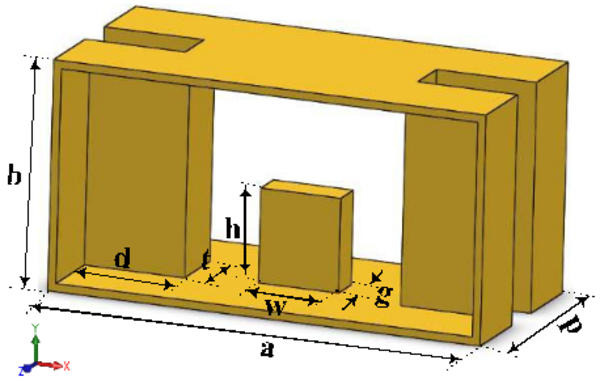
\includegraphics[width=0.95\linewidth]{figure/fig1}
	\caption{Schematic design of unit period of the SWS.}
	\label{fig1}
\end{figure}

\begin{figure}[phtb]
	\centering
	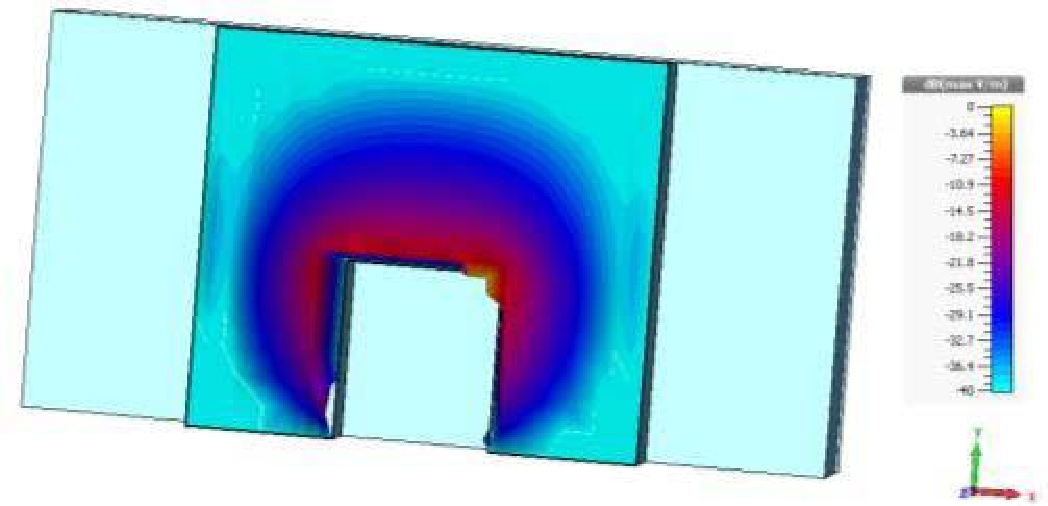
\includegraphics[width=0.95\linewidth]{figure/fig2}
	\caption{Fundamental mode axial electric field component on transverse cross section for phase, 2.5$ \pi $.}
	\label{fig2}
\end{figure}

值得注意的是,由于$H$面和$E$面波纹的原因,可以使用多种几何参数的剪裁来轻松地完成器件指标的优化。所选择的SWS横向尺寸$ a $和$ b $与标准矩形波导WR-2横截面尺寸兼容。 SWS和波纹几何参数的周期被优化以实现400\,GHz工作中心频率、线性色散曲线和低束压。设计参数如表\ref{tab:1}所示。这种结构可以用可用微细加工工艺的最小特征尺寸实现,如LIGA、DRIE和计算机数控纳米加工技术[25]。
\begin{table}[htbp]
	\caption{盒型窗计算参数}
	\centering
	\begin{tabular}{cc}
		\toprule
		Parameters & Dimension($ \mu $m) \\ \midrule
		$ a $    &         520         \\
		$ b $    &         254         \\
		$ p $    &         240         \\
		$ w $    &         100         \\
		$ g $    &         40          \\
		$ h $    &         113         \\
		$ d $    &         115         \\
		$ t $    &         60          \\ \bottomrule
	\end{tabular}
	\label{tab:1}
\end{table}
\section{电磁波特性} \label{sec:3}
为了研究该$H$面和$E$面加载的SWS的电磁波特性,考虑了一个周期的SWS。单周期的两个纵向边上施加Floquet边界条件。在一个周期内扫描波的相位值时,利用CST微波工作室的本征求解器得到相应的频率和波场成分。

图\ref{fig3}给出了表\ref{tab:1}中确定的SWS参数的TE$ _x $基模和第二模的色散曲线。SWS支持一系列空间谐波,其正向空间谐波必须作为TWT放大器的工作模式。在基模中,获得了345-455\,GHz的通带频率范围。在第一个正向空间谐波(相位,$2.5 \pi - 3\pi $)中,17\,kV的束线在350-440\,GHz频率范围内截断色散曲线。从图\ref{fig3}中非常宽的截取中可以看出行波管的瞬时带宽较大。在SWS的变化周期长度$ p $上,基波一次谐波的同步电压如图\ref{fig4}所示。对于确定的设计参数,在宽带上实现了恒定的电子束电压,以与波束互作用的波形同步。而且,观察到随着周期长度的减小,束电压降低。

\begin{figure}[phtb]
	\centering
	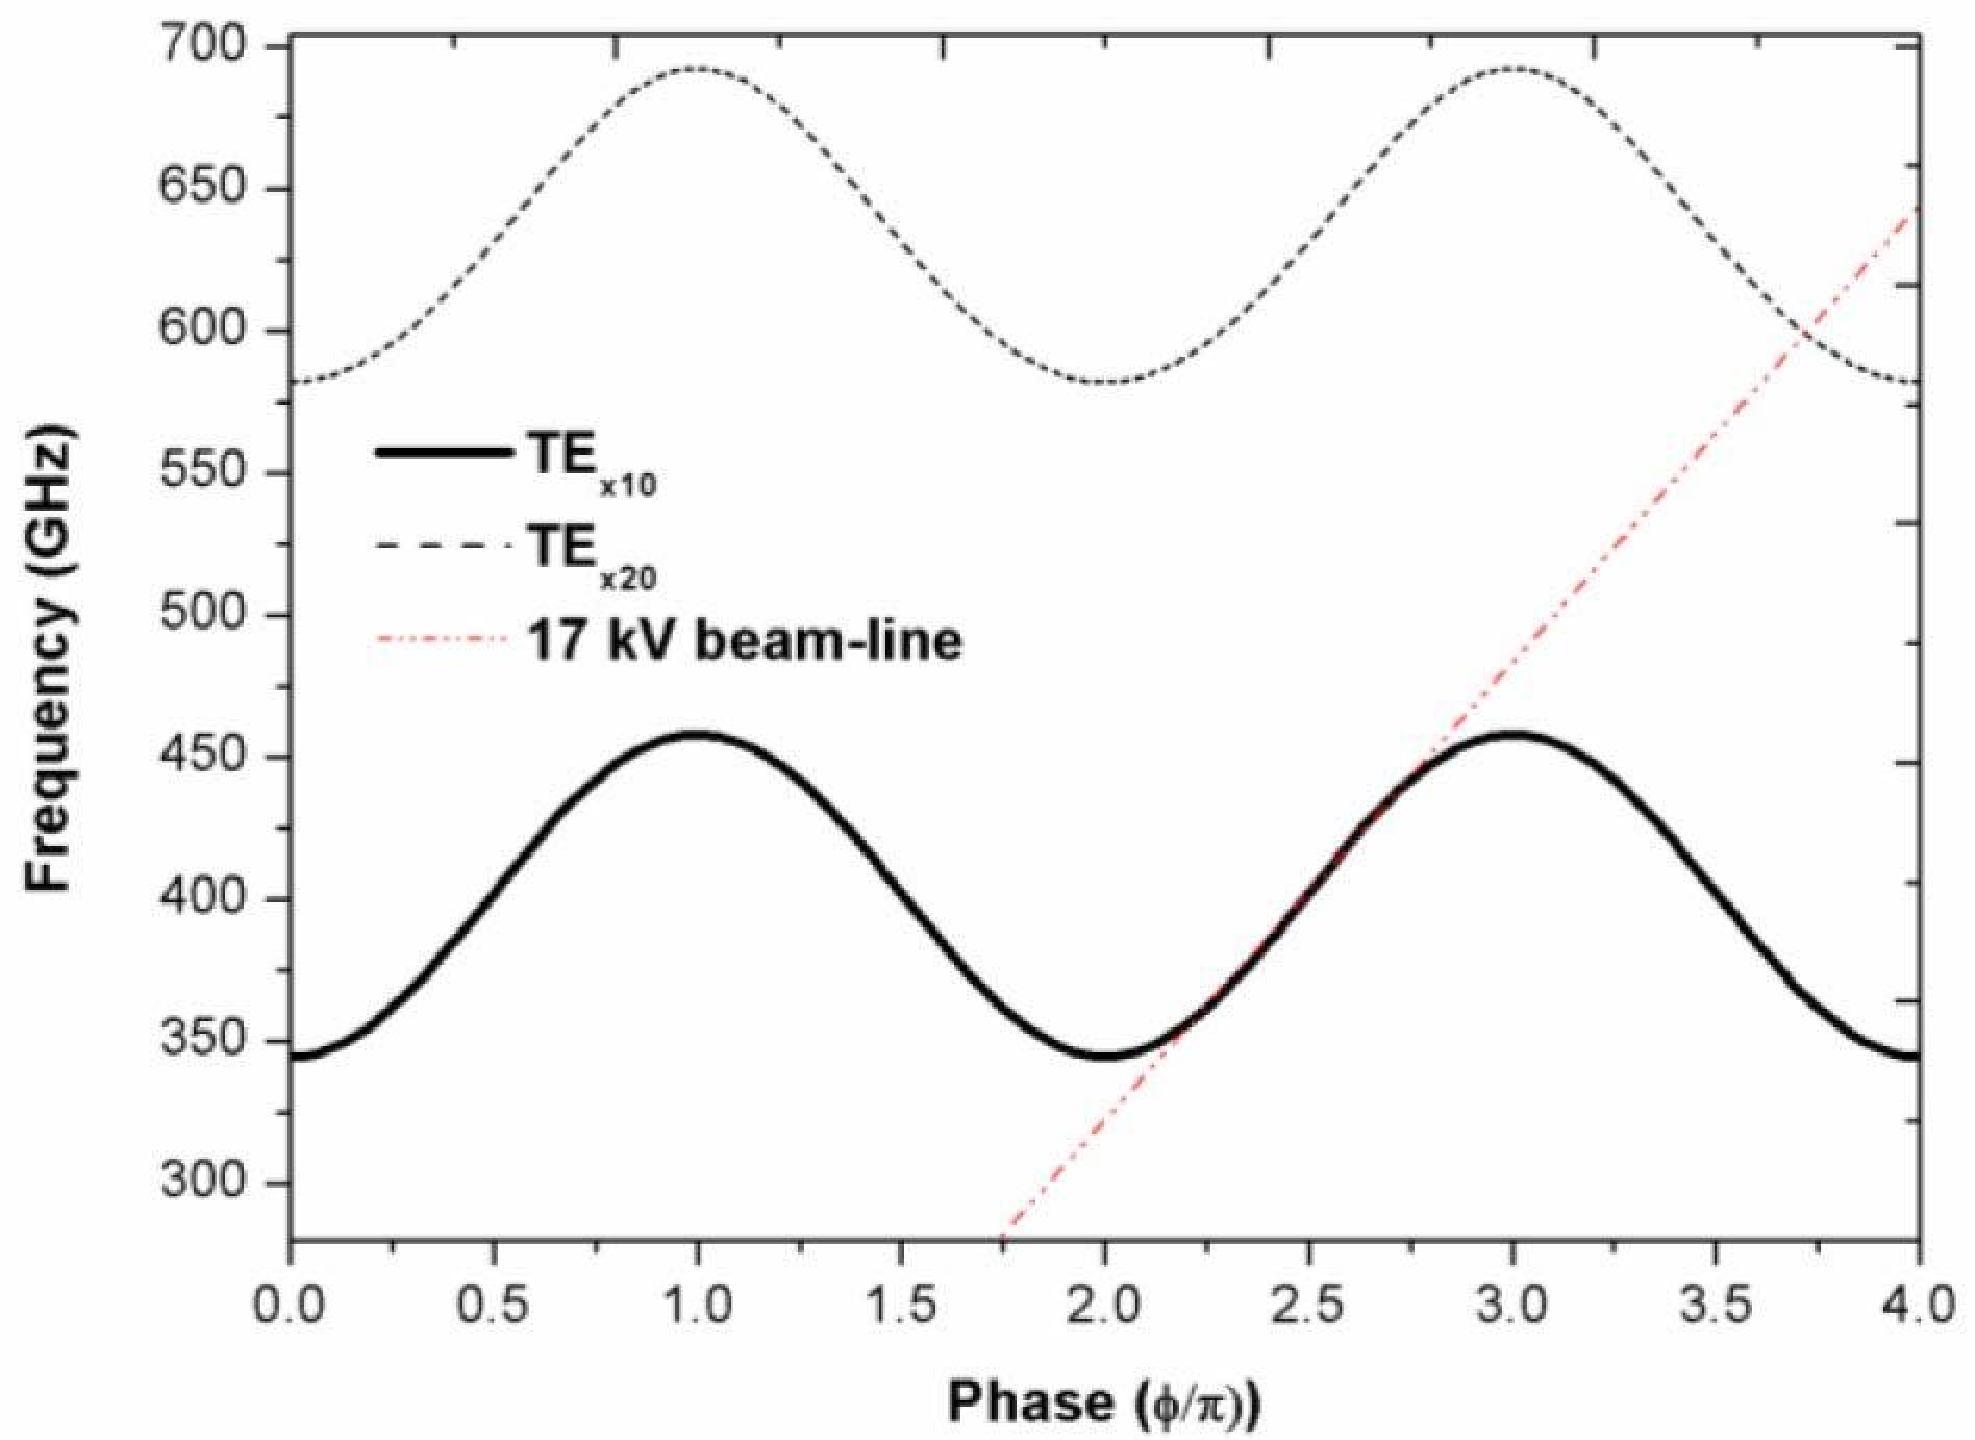
\includegraphics[width=0.95\linewidth]{figure/fig3}
	\caption{Dispersion curve for fundamental mode (TE$ _{\times 10} $) and second mode (TE$ _{\times 20} $).}
	\label{fig3}
\end{figure}

\begin{figure}[phtb]
	\centering
	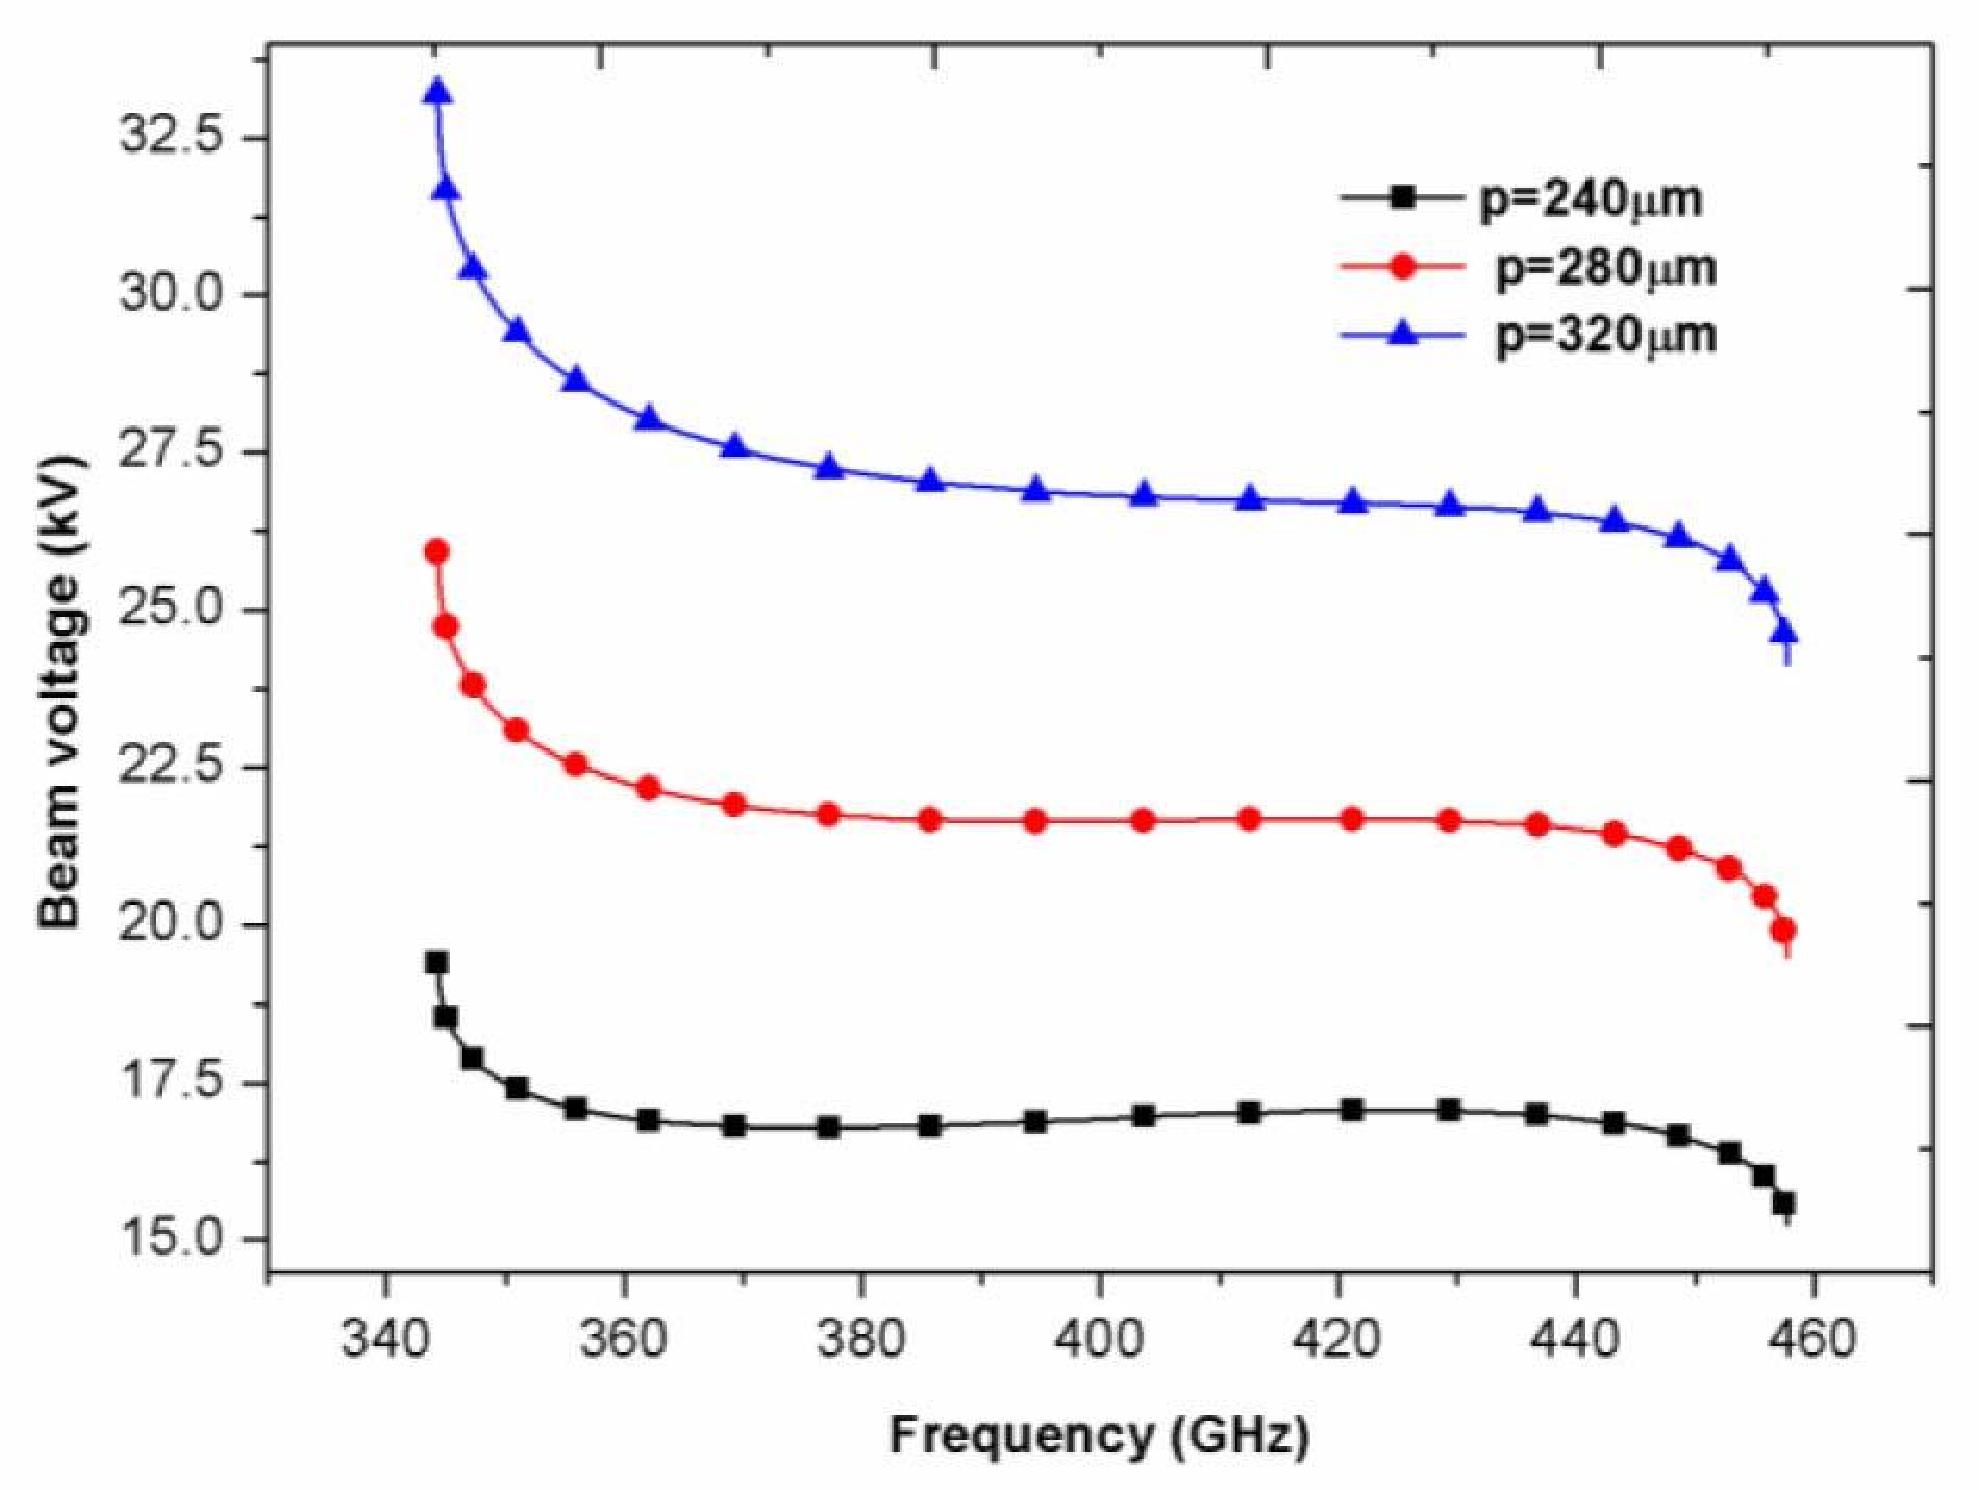
\includegraphics[width=0.95\linewidth]{figure/fig4}
	\caption{Beam voltage for varying period $ p $, other parameters kept constant.}
	\label{fig4}
\end{figure}


SWS的一个重要目标是获得最大化的耦合阻抗,它是注-波互作用有效性的量化参数。 SWS的耦合阻抗越大,器件的增益和输出功率就越高。第$ n $个空间谐波的耦合阻抗由下式给出
\begin{equation} \label{eq:1}
K_{cn}= \frac{\int \limits _S \vert E_{zn}\vert ^2}{2\beta_n^2P_{wg}}
\end{equation}

其中$ $E$_{zn} $是第$ n $个空间谐波纵向电场系数,$ \beta_n $是第$ n $个空间谐波数,$ P_{wg} $是横截面的平均功率,$ S $是电子注横截面面积。根据可用的互作用场强度,带状注横截面的几何参数被优化到 $100 \mu \textrm{m} \times 60 \mu \textrm{m}$ ,并位于$E$面波纹上方$ 40 \mu\textrm{m} $处。图\ref{fig5}是$ H $面加载对结构性能的潜在影响,特别是通过改变$H$面波纹参数$ d $和$ t $来研究其耦合阻抗。在基模的正向波一次谐波中,对于确定的带状注参数评估了其耦合阻抗。有意思的是,通过分别增大$ d $和$ t $的值,观察到耦合阻抗亦随之增加,同时通带范围随之降低。因此,推断$H$面加载增强了耦合阻抗,由此使得器件具有更高增益和输出功率——尽管是在减小工作带宽的条件下。
\begin{figure}[phtb]
	\centering
	\subfloat[]{
		\label{fig5-1}
		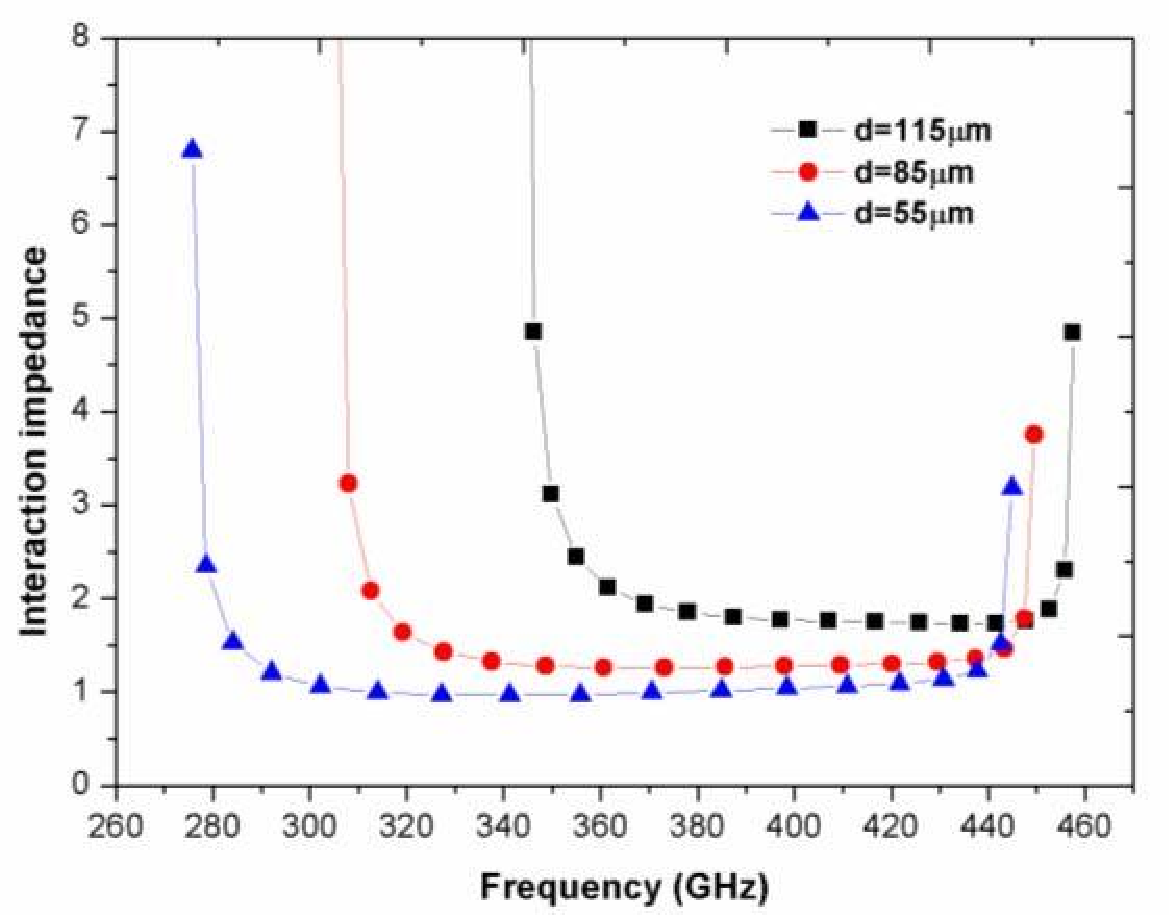
\includegraphics[width=0.95\linewidth]{figure/fig5-1}
	}
	\\
	\subfloat[]{
		\label{fig5-2}
		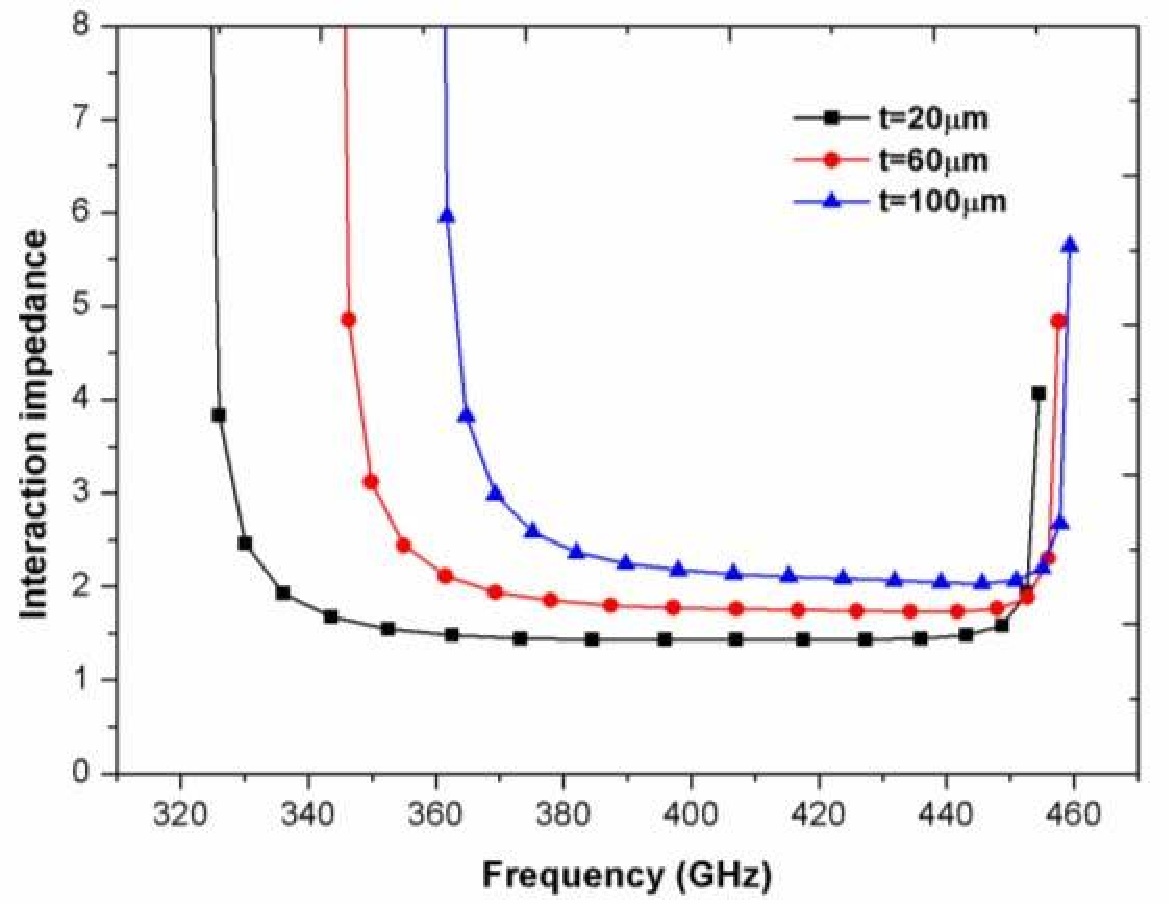
\includegraphics[width=0.95\linewidth]{figure/fig5-2}
	}
	\caption{Interaction impedance for varying H-plane corrugation dimensions. (a) Width $ d $. (b) Thickness $ t $.}
	\label{fig5}
\end{figure}

研究SWS中的传导损耗是很重要的,因为在THz体系中,波的趋肤深度约为几百纳米。实际上,在微细加工中要实现完美光滑的金属壁非常困难。考虑到金属壁的表面粗糙度,电磁波将遭受严重的衰减,这对于最小化以实现期望的功率和增益非常关键。金属的有效电导率作为表面粗糙度的函数由下式计算[26]:
\begin{equation} \label{eq:2}
\sigma_{\mathrm{eff}} = \frac{\sigma}{\left( 1+\exp\left( -\left( \frac{\delta}{2R_q}\right)^{1.6}\right) \right)^2  }
\end{equation}
其中$ \delta $是趋肤深度,$ R_q $是rms表面粗糙度,$ \sigma $是纯金属的电导率。计算了不同表面粗糙度下金属的有效导电性。图\ref{fig6}显示的是以dB/周期为单位的导电损耗,它由$ \alpha = \omega/\left(2QV_g\right) $算得,其中$ \omega $是本征频率,$ Q $和$ V_g $分别是扰动的$ Q $因子和群速。可见,表面粗糙度越高,导电损耗越大,对于65 nm的表面粗糙度,同理想的光滑金属壁相比,其导电损耗将增加到50\%。
\begin{figure}[phtb]
	\centering
	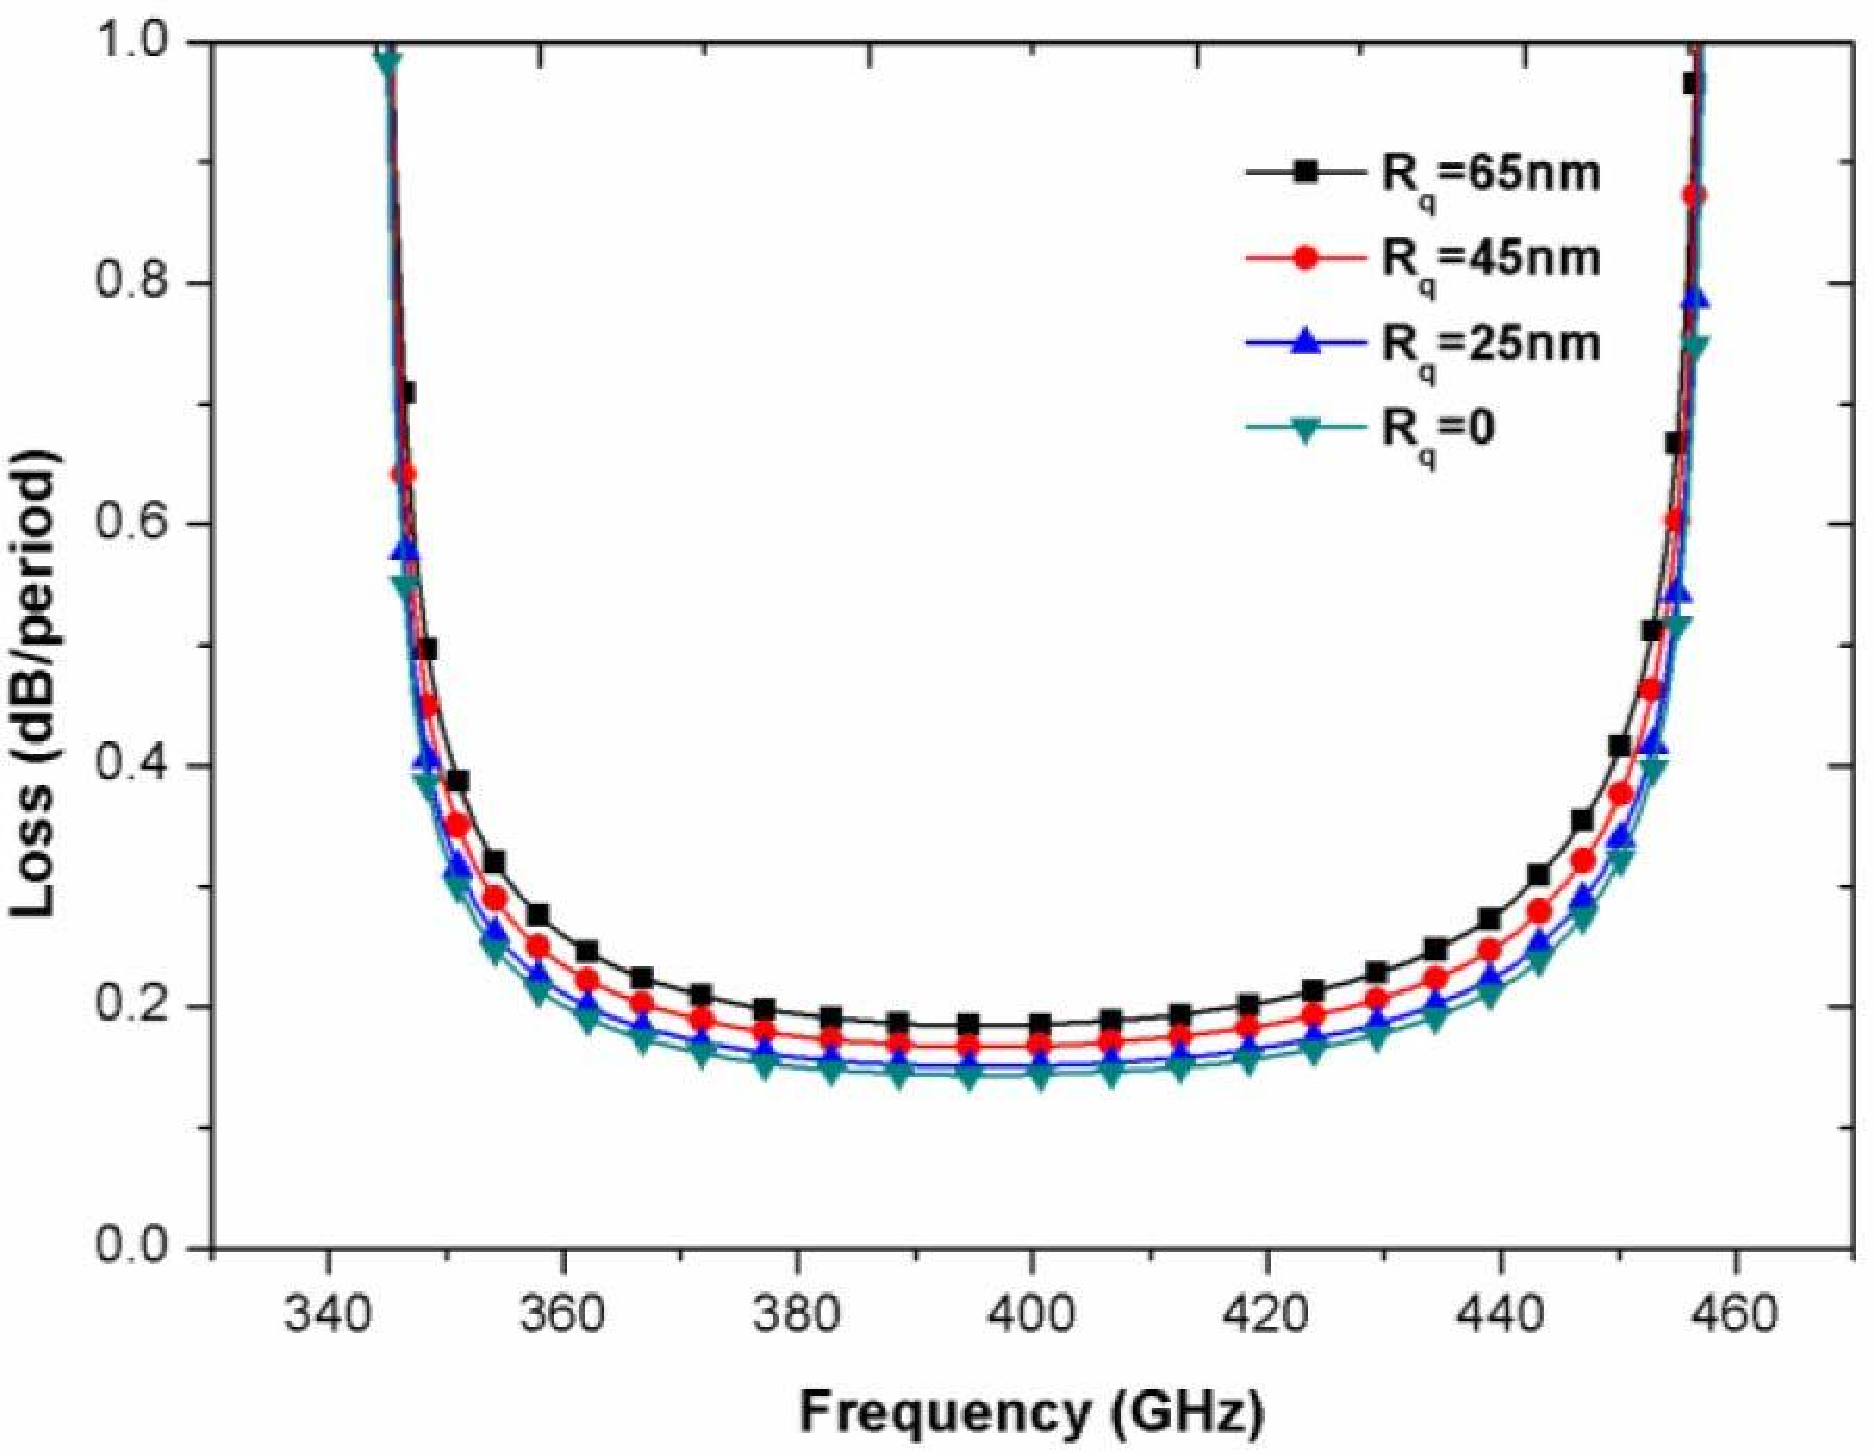
\includegraphics[width=0.95\linewidth]{figure/fig6}
	\caption{Loss in dB/period for different values of surface roughness.}
	\label{fig6}
\end{figure}

\section{注-波互作用} \label{sec:4}

从第\ref{sec:3}节中已知的电磁特性,如色散、电子束电压、改善的互作用耦合阻抗和互作用结构的损耗等,可用PIC求解器和CST来对行波管的性能做出预测。 行波管的注-波示意图如图\ref{fig7}所示。我们在互作用结构中采用了90个周期,长度为21.6\,mm。为了使来自输入端口和输出端口的反射最小,并使其与快波和慢波之间的波的过渡相兼容,输入和输出耦合器被设计为$E$面垂直的波纹高度和$H$面水平的波纹宽度均渐变(渐缩)的结构,其渐变长度为19个周期。带耦合器和完整互作用结构的反射(S$ _{11} $)和透射(S$ _{21} $)系数在通带频率范围内显示出良好的波传播特性,如图\ref{fig8}所示。为了避免仿真模型过于复杂,电子枪通过将电子发射表面设置为具有17\,kV束压和20\,mA束流的电子束来简化。根据电子束的横截面来优化束流,并减小空间电荷效应。为了限制沿着传播路径的电子束运动,纵向施加0.6\,T的均匀磁场聚焦。假定金属表面粗糙度为65\,nm,此时计算出的有效电导率$ 3.6\times 10^7\,\Omega^{-1}\mathrm{m}^{-1} $ 被定义为金属壁的实际电导率,假定的表面粗糙度可通过微细加工技术来实现。通常,对注-波互作用的三维PIC模拟会消耗更多的计算机资源,并且需要更长的模拟时间。因此,对纵向电场进行网格优化。该设置模型在仿真结束时具有310万个网格单元和$ 57\times 10^6 $个粒子。

\begin{figure}[phtb]
	\centering
	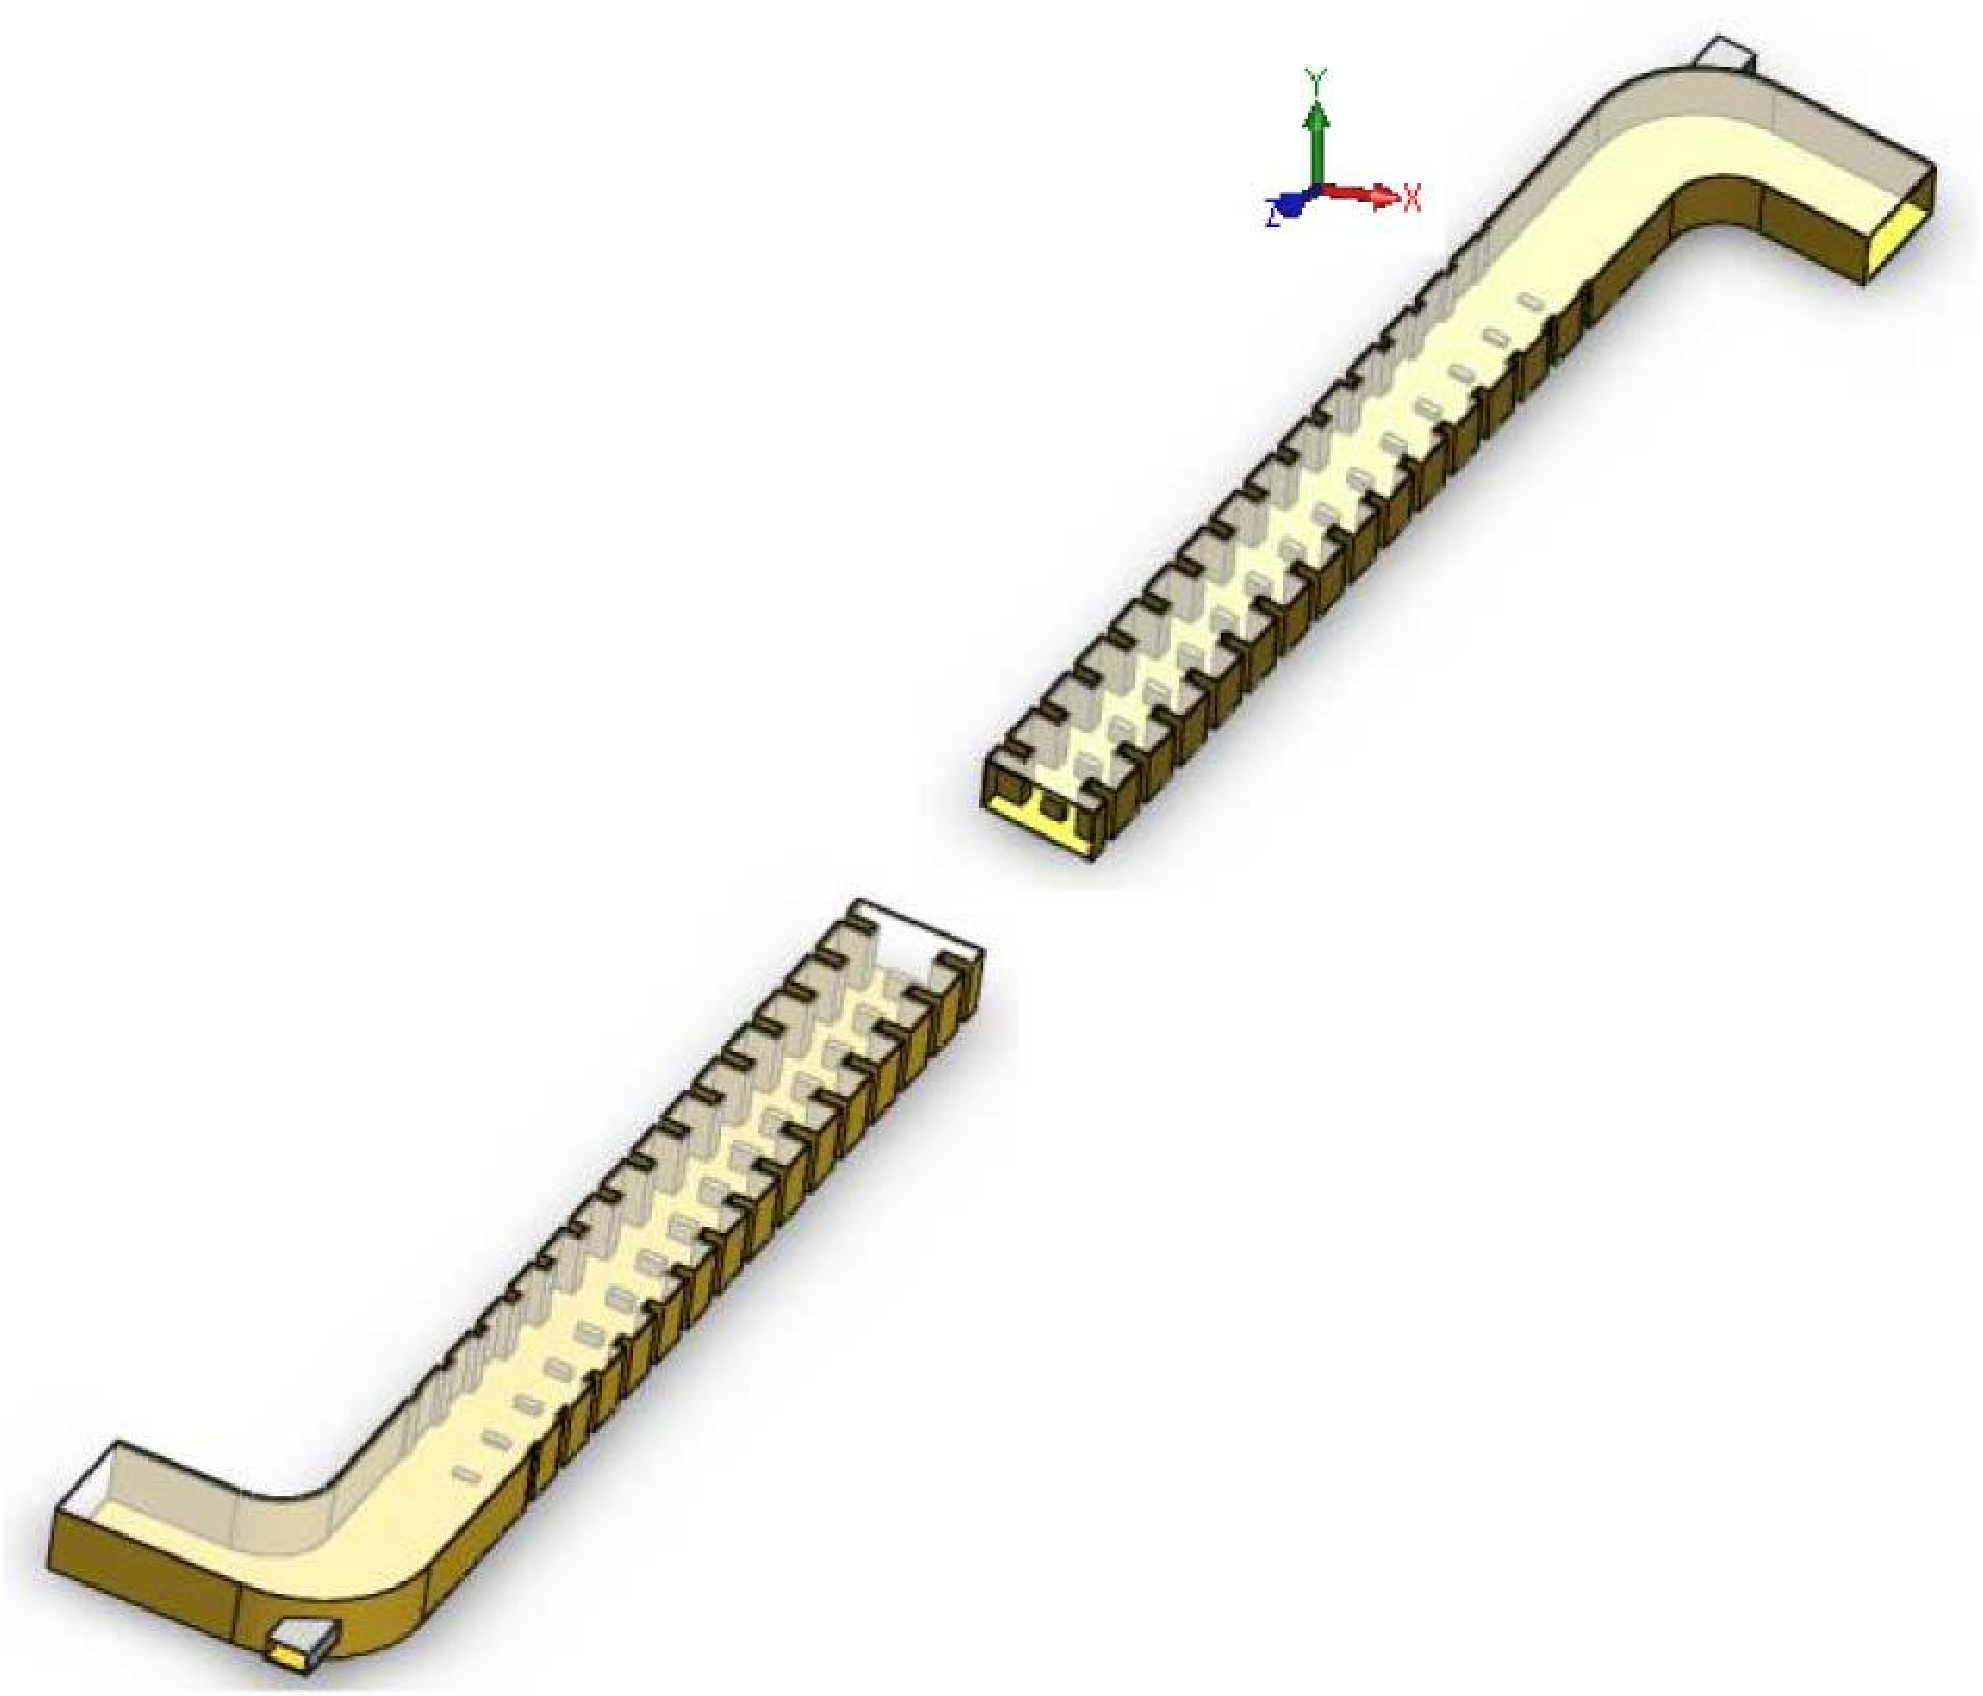
\includegraphics[width=0.95\linewidth]{figure/fig7}
	\caption{Schematic of H-plane and E-plane loaded SWS-based TWT amplifier.}
	\label{fig7}
\end{figure}

\begin{figure}[phtb]
	\centering
	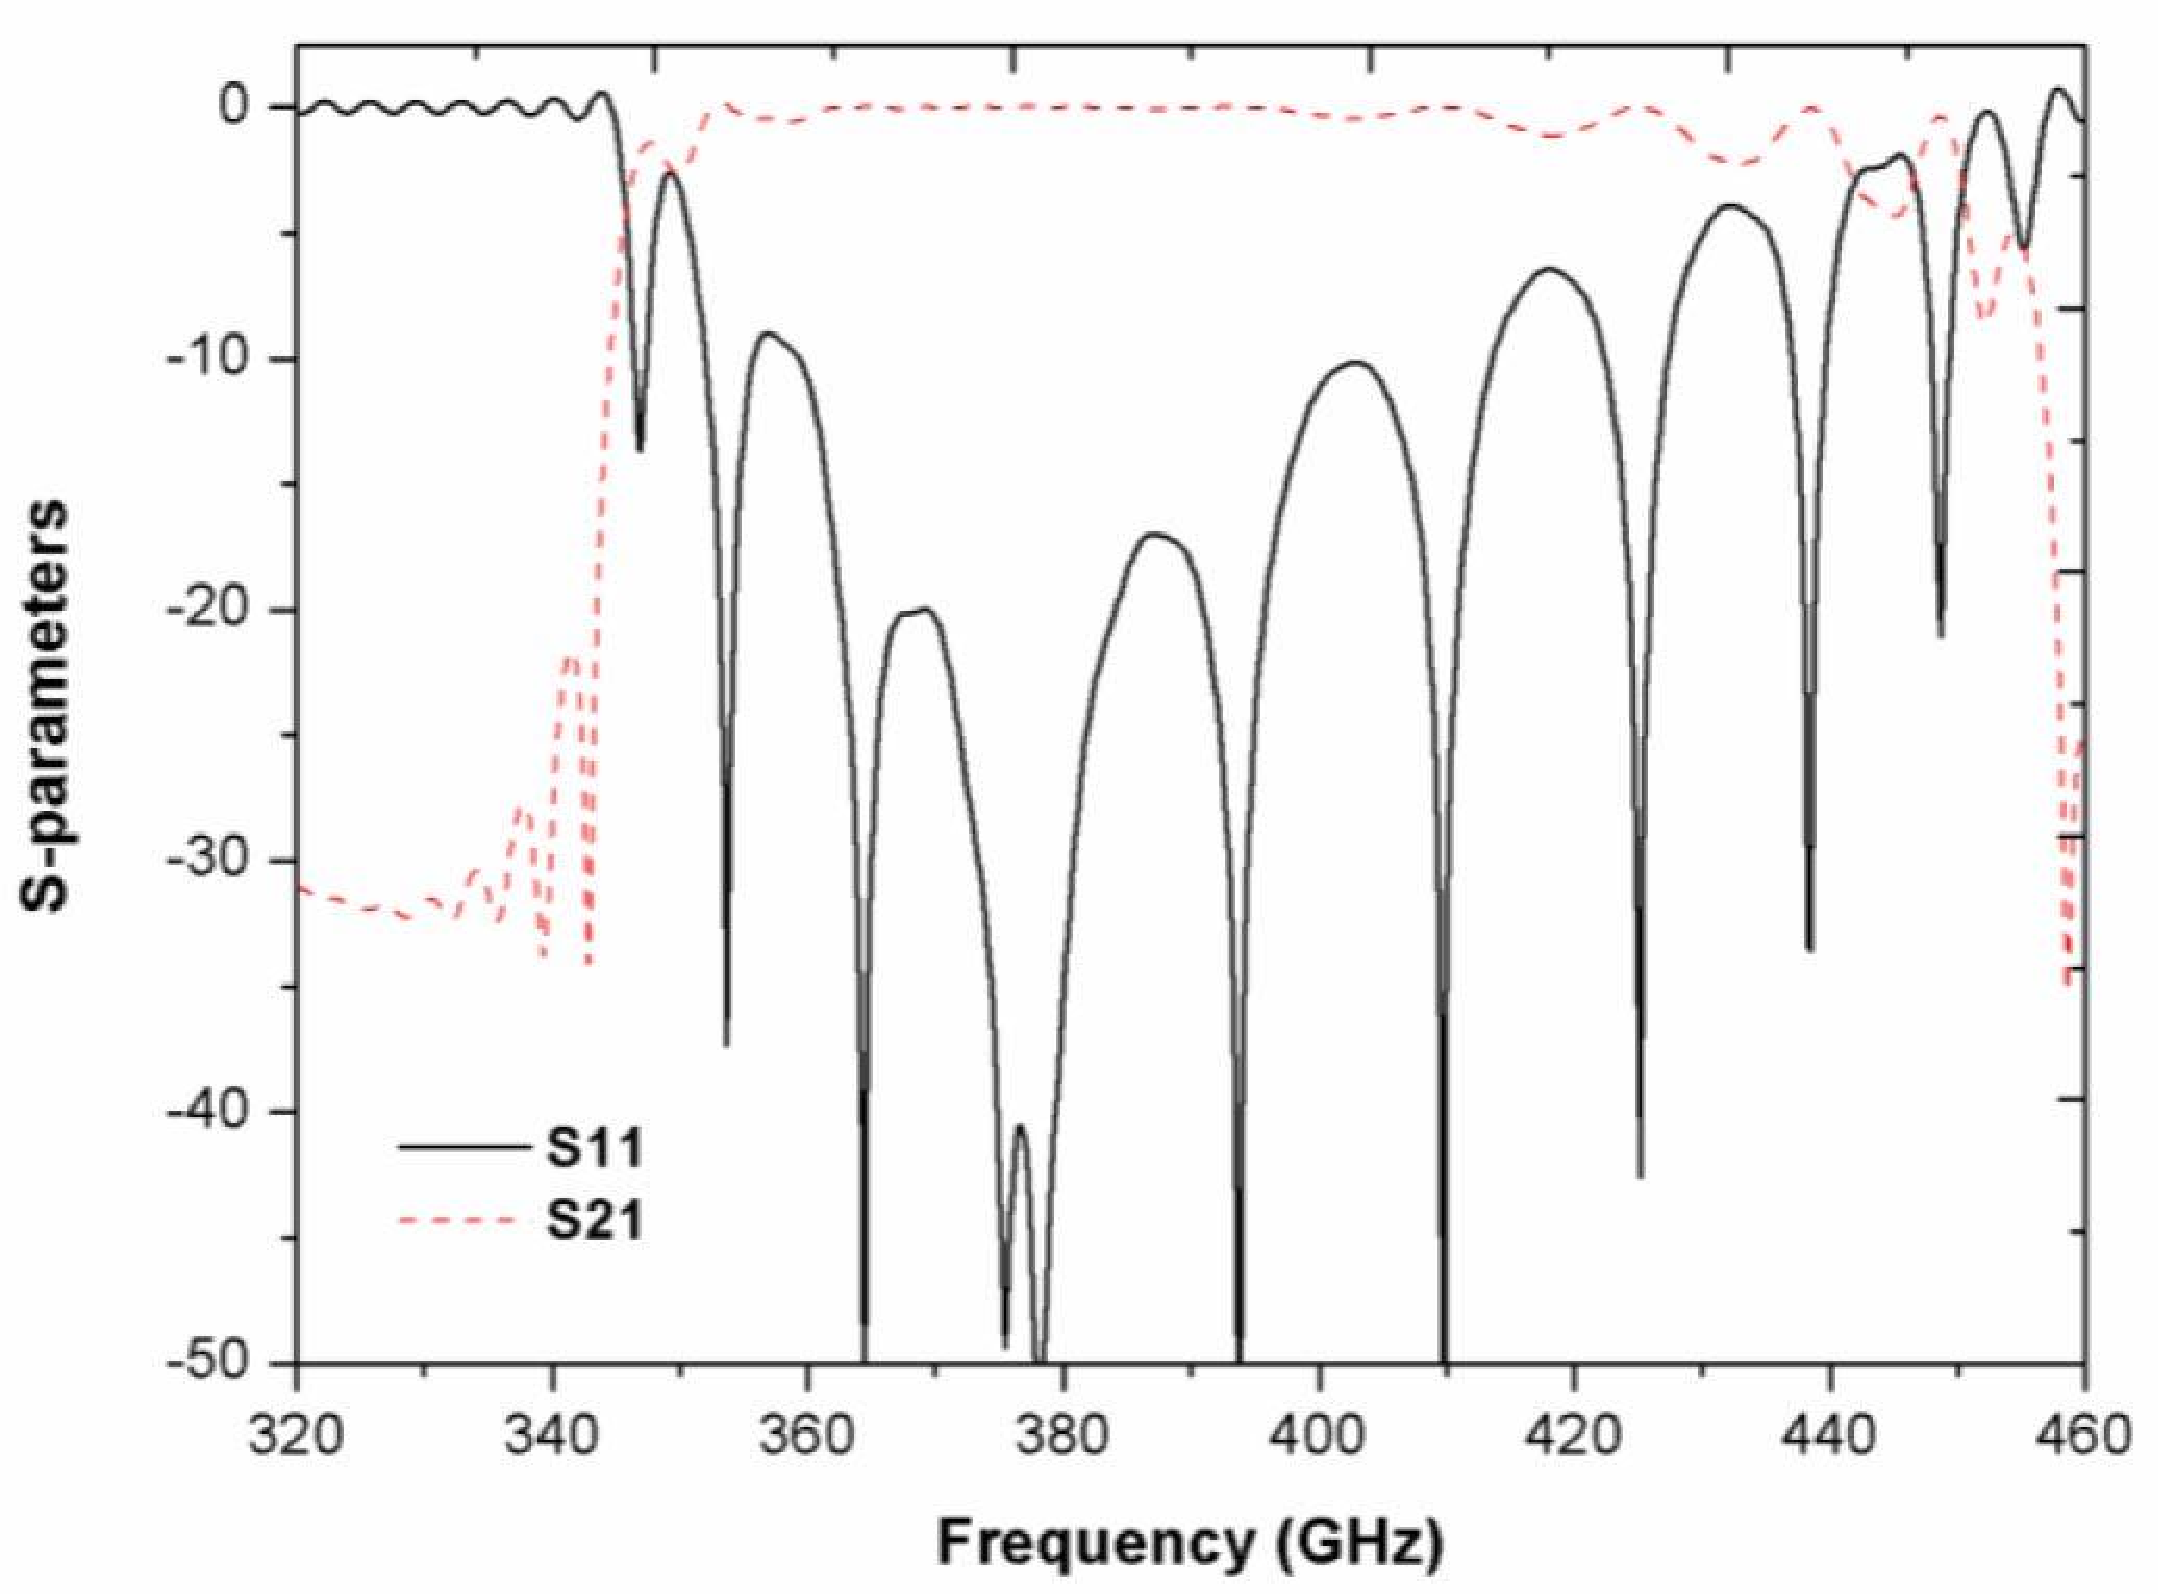
\includegraphics[width=0.95\linewidth]{figure/fig8}
	\caption{S-parameters of interaction structure with input and output couplers.}
	\label{fig8}
\end{figure}


本文所提出的行波管的小信号增益计算是针对所施加的50\,mW输入功率的连续波(CW)激励信号来执行的。图\ref{fig9}显示了400\,GHz激励下的输入和输出信号。 2\,ns后观察\newpage \noindent 到稳定的输出信号,增益为19.5\,dB,输出功率为4.6\,W。使用E5530 Xeon处理器(2.8\,GHz,72\,GHz\footnote{原文如此,疑为GB(译注)}存储器),对于6\,ns仿真,计算时间为73\,h。为了预测放大器的瞬时带宽,在每个模拟运行的通带上的离散频率点处执行模拟。图\ref{fig10}示出了在355-435\,GHz的频率范围内实现了80\,GHz的瞬时带宽。下限和上限截止频率通带中的增益下降是由于来自输入和输出端口的波反射以及与电子注同步时的损失。 在瞬时带宽上获得超过0.9\%的电子效率。电子注速度与SWS长度之间的函数关系如图\ref{fig11}所示。当电子注沿着传播方向移动时,它和电磁波之间的连续互作用导致聚束了的电子注速度的降低,最终在管子末端注-波不再同步。相速渐变技术可以使注-波的速度再次同步,这有助于提高总体注-波互作用效率。对于400\,GHz激励的高输入功率也进行了大信号模拟,如图\ref{fig12}所示。由于这种器件的非线性特性,输出功率饱和到大约19.3\,W。

\begin{figure}[phtb]
	\centering
	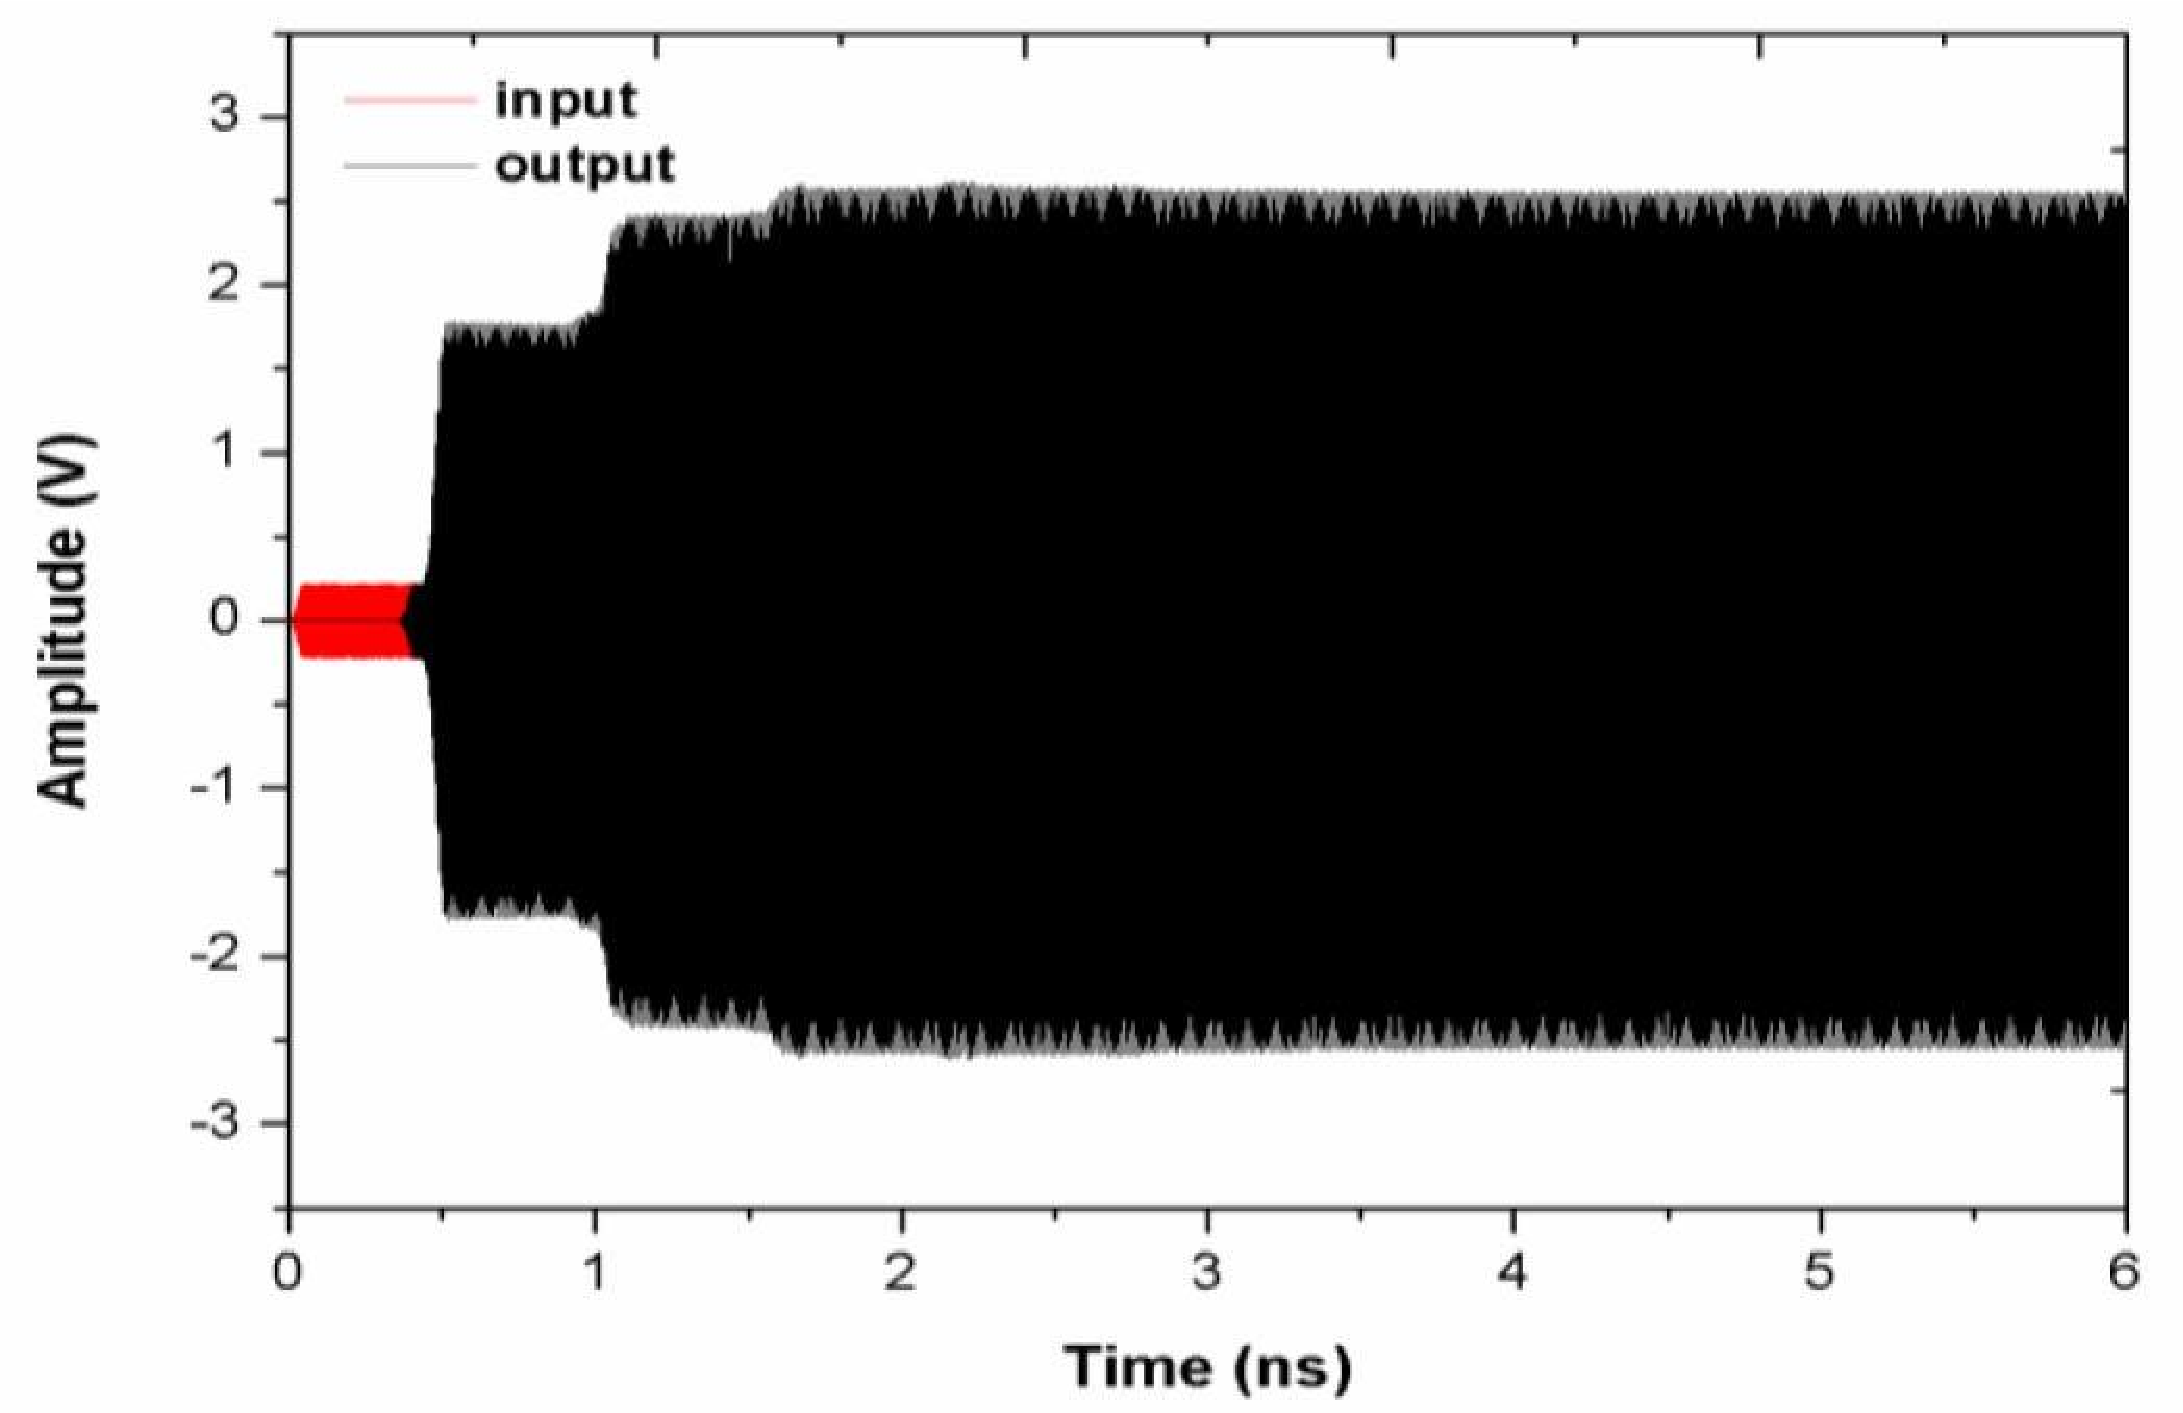
\includegraphics[width=0.95\linewidth]{figure/fig9}
	\caption{Input and output signals for 400-GHz CW excitation with 50-mW
power.}
	\label{fig9}
\end{figure}


\begin{figure}[phtb]
	\centering
	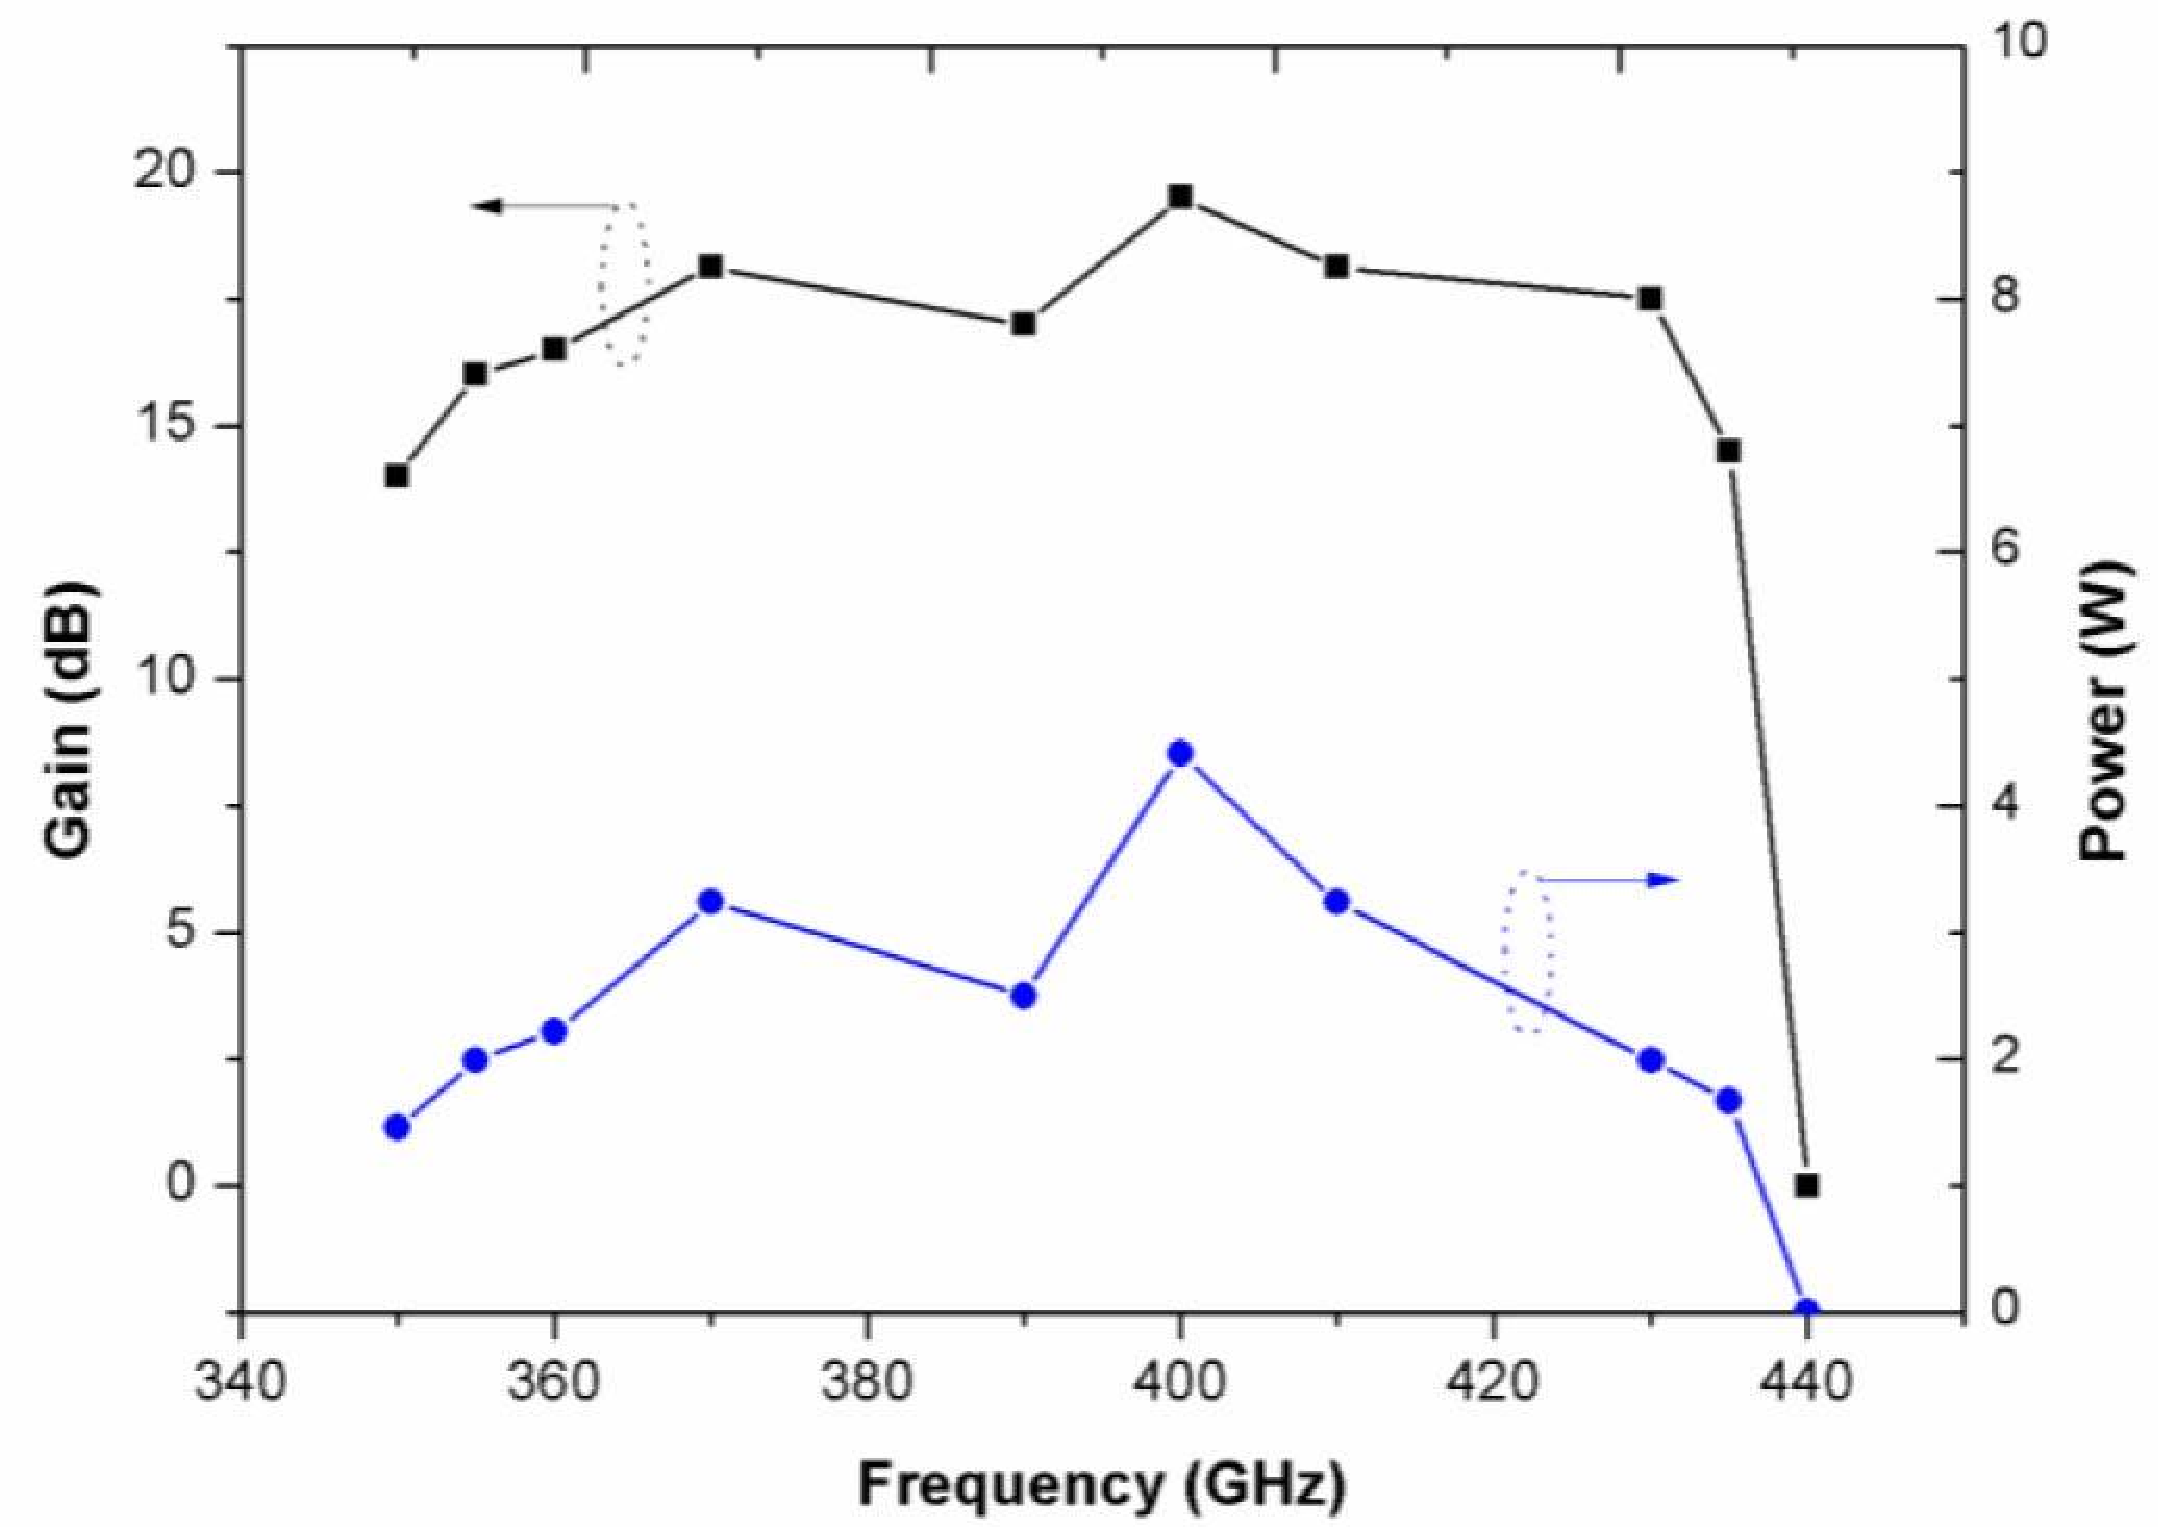
\includegraphics[width=0.95\linewidth]{figure/fig10}
	\caption{Gain and output power versus CW excitation frequency of 50 mW}
	\label{fig10}
\end{figure}


\begin{figure}[H]
	\centering
	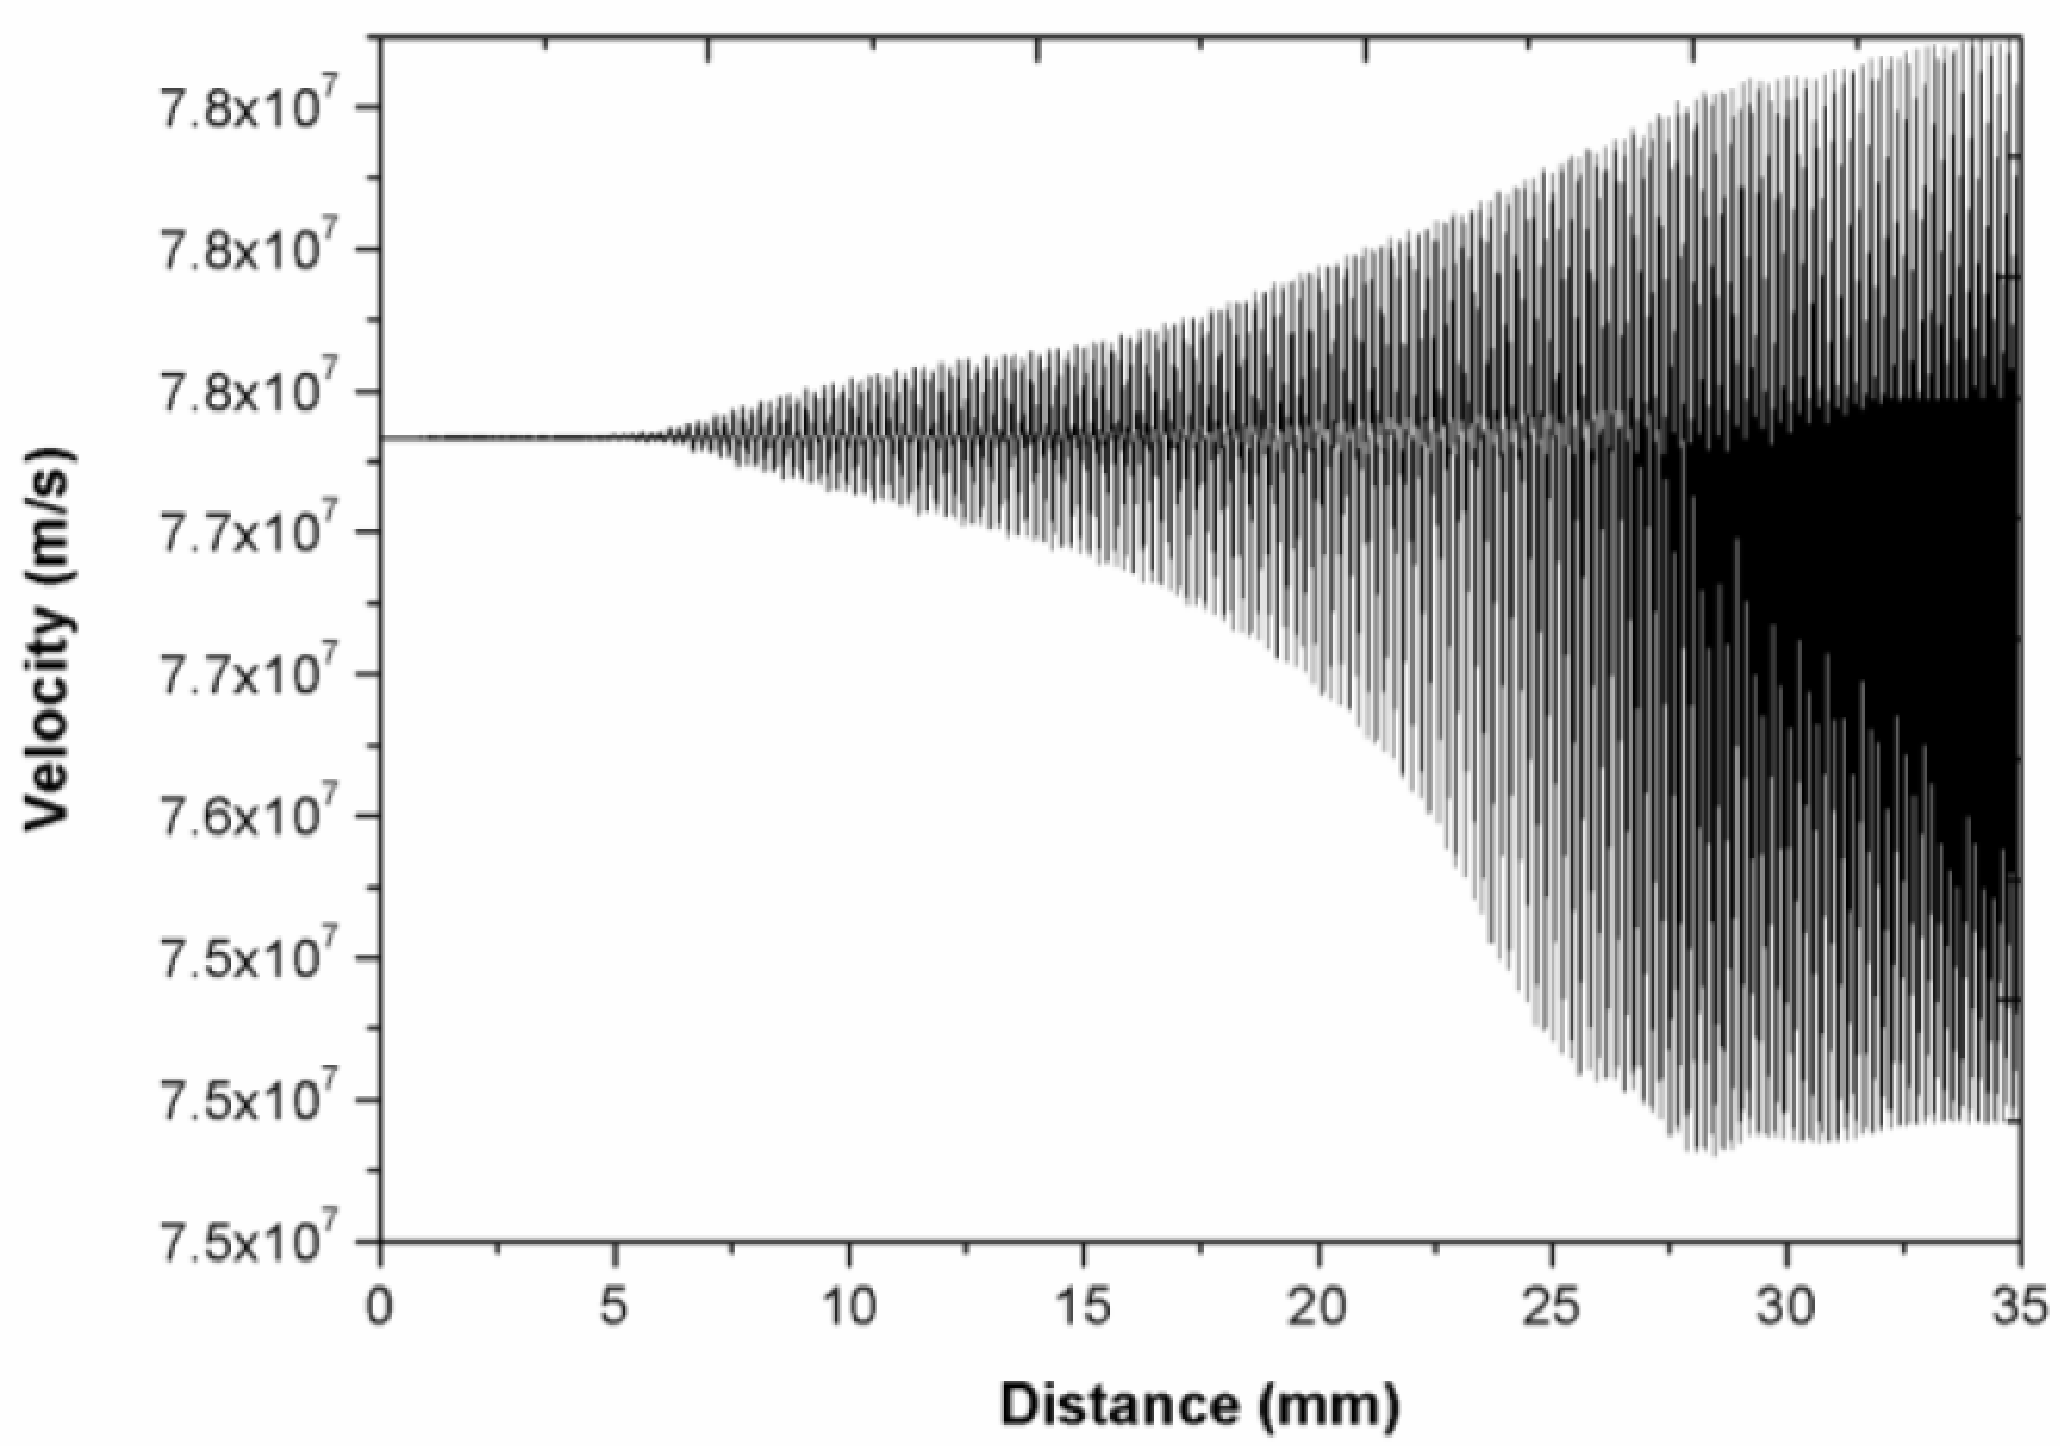
\includegraphics[width=0.95\linewidth]{figure/fig11}
	\caption{Beam velocity as a function of the SWS length for 400 GHz.}
	\label{fig11}
\end{figure}


\begin{figure}[H]
	\centering
	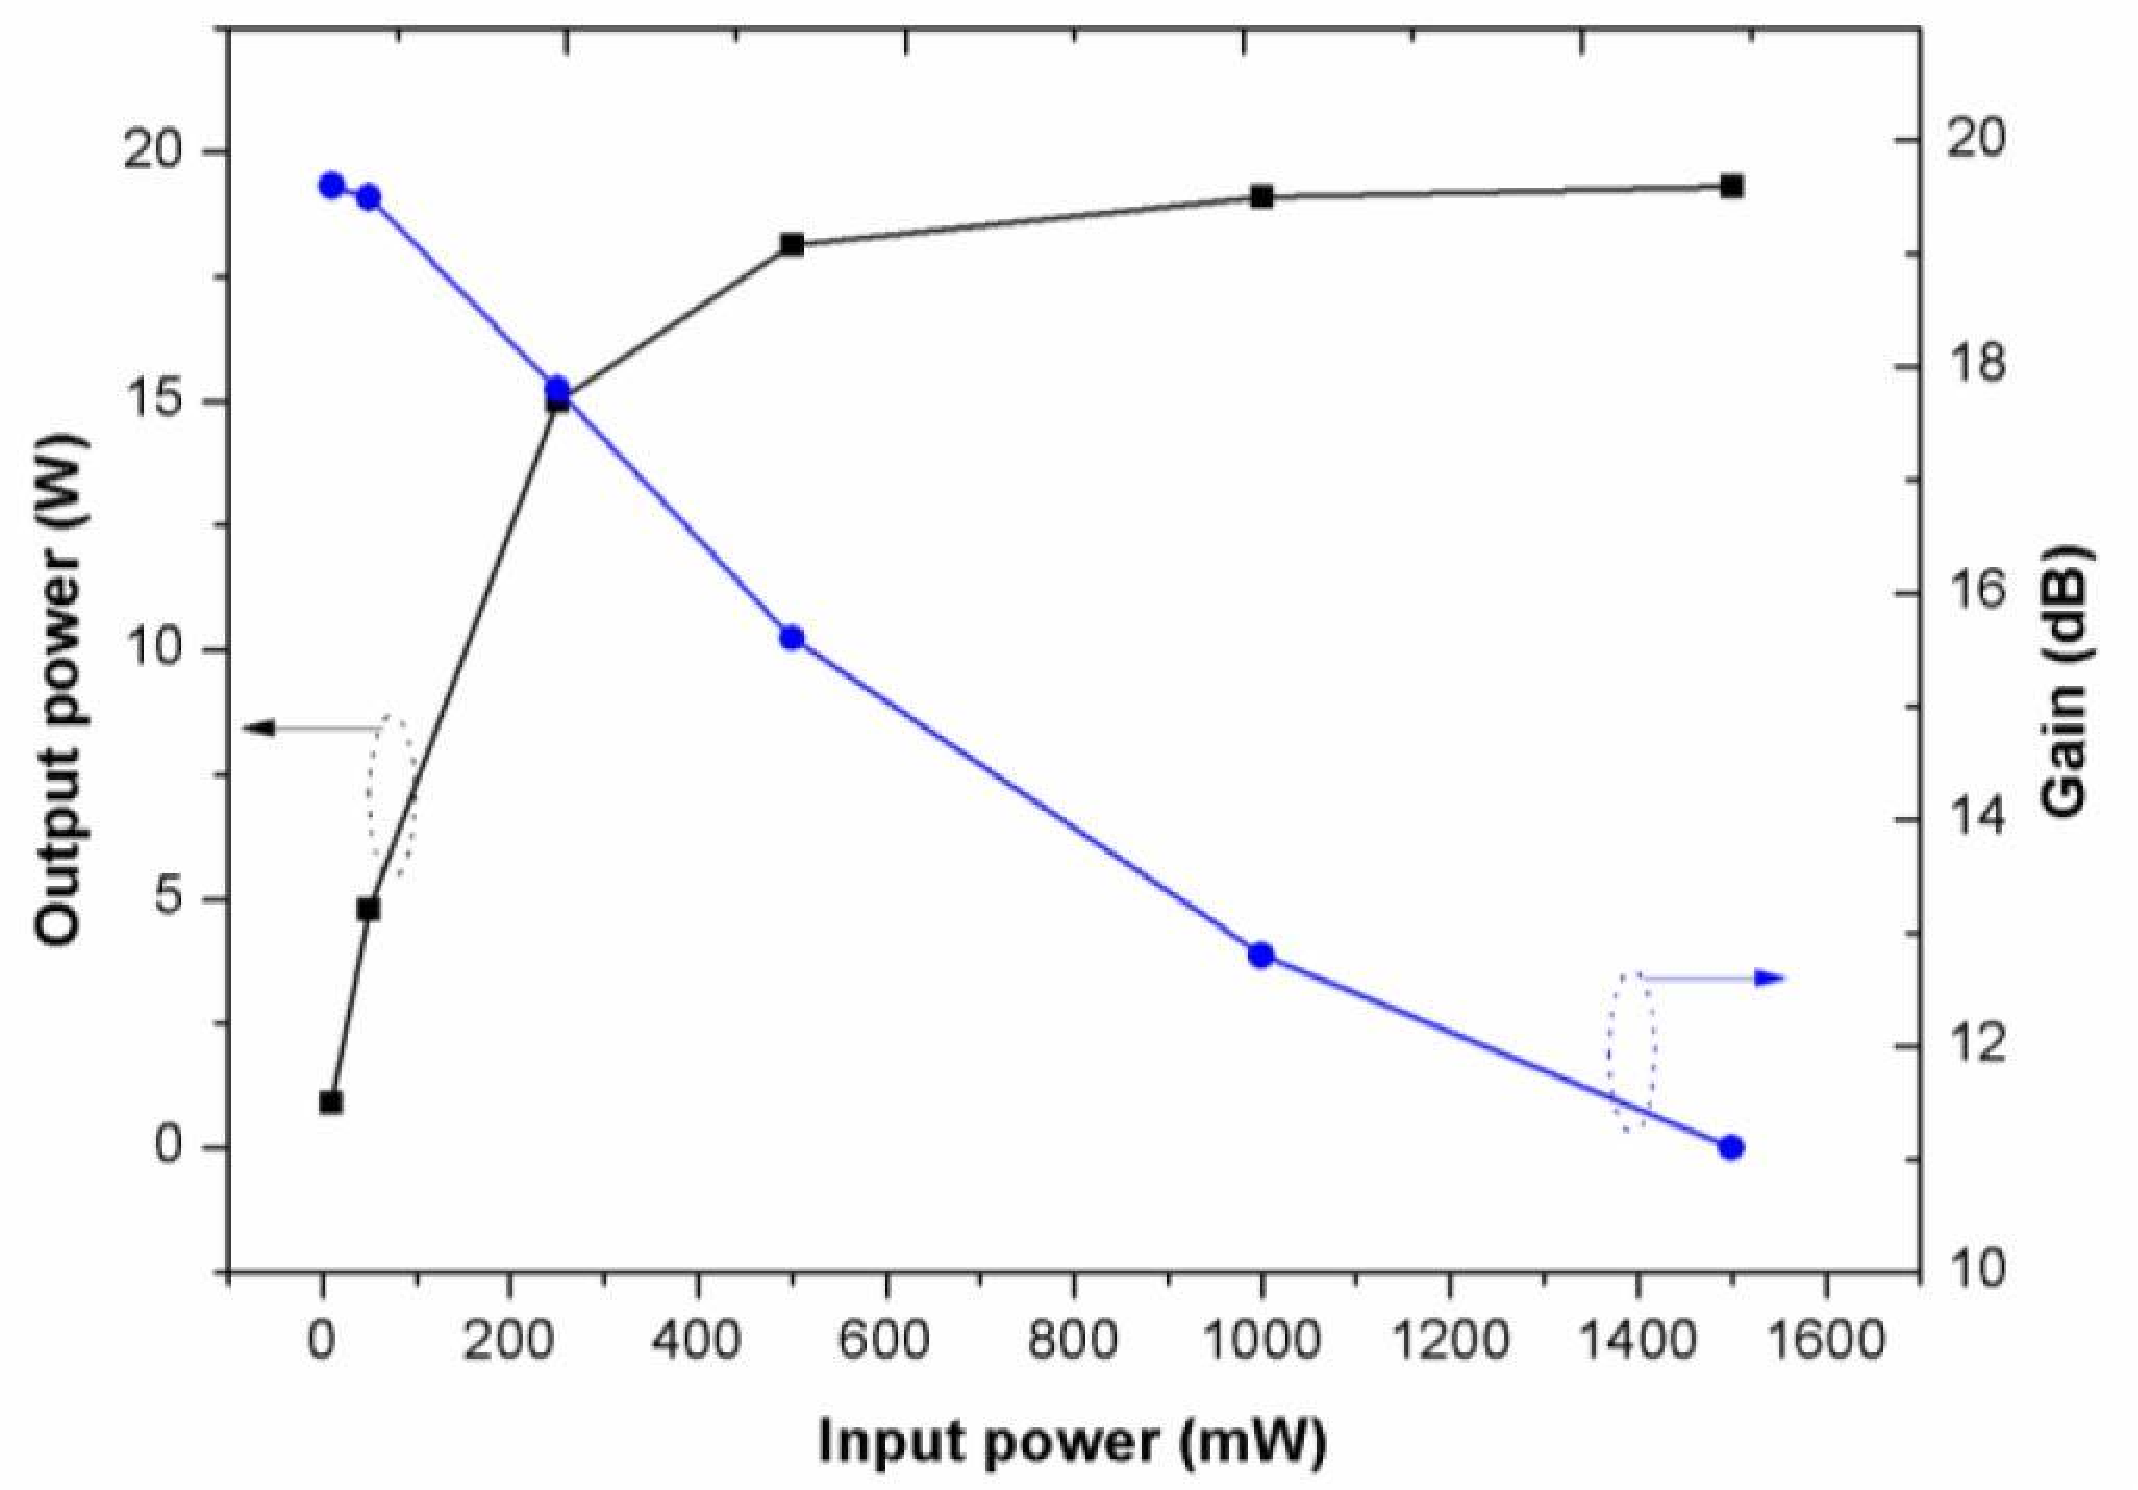
\includegraphics[width=0.95\linewidth]{figure/fig12}
	\caption{Output power and gain versus input power of 400-GHz CW}
	\label{fig12}
\end{figure}

\newpage
\section{结论} \label{sec:5}
$H$面和$E$面加载的慢波电路已经被证明是用于中心频率为400\,GHz的行波管放大器的新型SWS。有趣的是,除了SWC中通常的$E$面负载之外,还通过采用$H$面负载获得增强的互作用耦合阻抗。考虑到众多设计参数的灵活性,SWS给出了与电子注能宽频带同步的线性色散曲线。该注-波互作用模拟显示出了有希望的TWT放大器性能,例如80\,GHz的瞬时带宽,对于400\,GHz、固定为17\,kV的中等束压和20\,mA的束流下,最大增益为19.5\,dB。大信号模拟预测了400\,GHz连续激励的饱和输出功率为19.3\,W。所提出的结构拓扑和几何参数与最近的微细加工技术的特征尺寸很好地相容。基于仿真结果,本SWS的演示性能使其成为TWT器件的合适候选者。%\enlargethispage{-6.5cm}

\section*{Reference\footnote{注:本文为译文,相关参考文献见原文。原文文献信息如下:\href{http://ieeexplore.ieee.org/document/7426768/}{H-Plane and E-Plane Loaded Rectangular
			Slow-Wave Structure for Terahertz TWT Amplifier,IEEE TRANSACTIONS ON ELECTRON DEVICES, VOL. 63, NO. 4, APRIL 2016}\\(翻译人:李胜明)}}


\end{document}